\documentclass{kththesis}
\usepackage[utf8]{inputenc}
\usepackage{csquotes}
\usepackage[style=numeric,sorting=none,backend=biber]{biblatex}
\addbibresource{sources.bib}
\usepackage{url}
\usepackage{amsmath}
\usepackage{amssymb}
\usepackage{graphicx}
\usepackage{float}
\graphicspath{ { ./images/ } }
\usepackage{hyperref}
\hypersetup{
hidelinks
}

\title{}
\alttitle{Klassificering av hjärnaktivitet i Parkinsons Sjukdom}
\author{}
\email{}
\supervisor{Arvind Kumar}
\examiner{Pawel Herman}
\programme{Bachelor in Computer Science}
\school{School of Electrical Engineering and Computer Science}
\date{\today}
\kthcover{kth-cover.pdf}

\begin{document}

\frontmatter
\titlepage

\begin{abstract}

This project has been concerned with creating methods for feature extraction for the purpose of classification of brain activity in parkinsonian brains. 
Classification of LFP activity was based on feature vectors produced from the DFT of activity, and a heuristic-motivated visualization of these using the k-Means algorithm for prediction and classification.
These feature vectors were also subject to principal component analysis as a further means of feature extraction and classification, highlighting differences in brain regions. 
Classification of spiking activity was based on spiking rates, joint rate distributions, serial correlation coefficients, power spectral density, and spectral entropy.
\end{abstract}

\begin{otherlanguage}{swedish}
\begin{abstract}
\textit{Vissa korrekta översättningar okända.}
Detta projekt har syftat att skapa metoder för att utvinna särdrag och att klassifiera hjärnaktivitet i parkinsonska hjärnor.
Klassificering av lokal fältpotential baserades på särdragsvektorer producerade från DFT:n av aktivitet, och en heuristiskt motiverad visualisering av dessa användande k-Means algoritmen för förutsägning och klassificering.
Dessa särdragsvektorer analyserades även med principalkomponentanalys för att utvinna ytterligare särdrag samt för klassificering, vilket påvisade skillnader i olika regioner av hjärnan.
Klassificering av spetsaktivitet baserades på spetstakt, beroende taktfördelning, seriella korrelationskoefficenter, spektral effektdensitet, och spektral entropi.
\end{abstract}
\end{otherlanguage}

\tableofcontents

\mainmatter

\chapter{Introduction}

Parkinson's disease (PD) is a progressive neurodegenerative disorder of movement that is age-related. 
It affects tens of millions of people worldwide, and the frequency and associated socioeconomic burden of the condition are set to increase as the elderly population grows.

The disease is characterized by poverty of voluntary movements (akinesia), slowness and impaired scaling of voluntary movement (bradykinesia), muscle rigidity and tremor of the limbs at rest \parencite{DeMaags}.

The hallmark feature of PD is the degeneration of dopamine neurons in the basal ganglia (BG), which is the region of the brain responsible for functions such as learning or movement \parencite{Hammond}. 
The BG consists of a few interconnected nuclei: the striatum (STR), globus pallidus (GP), subthalamic nucleus (STN), and substantia nigra (SN). 
The dopamine deficiency leads to a cascade of functional changes in the basal ganglia circuitry, which are ultimately responsible for the development of the main features of PD.

\section{Purpose}

The purpose of this project is to attempt to find one or several methods for classification of the brain activity in patients with Parkinson's disease.

Furthermore this project aims to, to some extent, use any produced methods to evaluate differences is brain activity of different categories.
It is of interest to consider what differences any such methods show when comparing brain activity from different brain regions.
It is also of interest to make a similar comparison for the brain activity in different subjects.

\section{Delimitations}

The authors of this report are not well educated or experienced in studying brain activity.
The methods produced are mainly means to serve as a strong foundation for further research into deeper understanding of Parkinson's disease.
The authors attempt to describe and interpret output produced by the methods, but do so outside of any broader implications the methods have for the further study of Parkinson's disease.

No software used, or produced, either by others or by the authors, is subject to extensive formal verification within the scope of this project. 
The same is true for the datasets used within the scope of this project.
The datasets used are instead assumed to have been produced/recorded to a satisfactory quality for their uses within the scope of this project.

\section{Research questions}

\begin{itemize}
    \item How can effective methods for classification of brain activity in patients with Parkinson's disease be produced?
    \item How can such methods be used to distinguish between brain activity from different regions of brains in patients with Parkinson's disease?
    \item How can such methods be used to distinguish between brain activity from different patients with Parkinson's disease?
\end{itemize}

\newpage
\chapter{Background}

The most valuable contribution to the clarification of the functional changes occurring in PD has been provided by the animal models of the disease, particularly those applied to rodents and primates \parencite{Mallet}. 
In rodents, chronic and acute dopaminergic denervation (obtained by inflicting a selective lesion of the BG that mimics the effects of PD) leads to excessive beta oscillatory activity in the BG's LFP that can be suppressed by treatment \parencite{Mallet}.

We will attempt to observe such oscillations and synchronization in the dataset we have acquired for this project, which consists of several different measurements of brain activity in dopamine-depleted rodents. 
The used measurements of brain activity are:

\begin{itemize}
    \item Local Field Potential (LFP): electrical signals generated in nervous tissues by the summed and synchronous activity of the individual neurons in that tissue.
    \item Spiking activity (also called action potential), which is a rapid rise and fall in voltage or membrane potential across a neuron's membrane. We have it in the form of background unit activity (BUA) and signal unit activity (SUA).
\end{itemize}

They were recorded simultaneously from three previously mentioned different regions of the BG; globus pallidus, striatum, and subthalamic nucleus, in sessions of 100 seconds at a sampling frequency of 16000 Hz.

Therefore, for these parts of the BG we dispose of information on LFP and spiking activity; the data for each specific type of recording (e.g. LFP in the GP), for a specific animal and recording session will be called a “channel”. 
These continuous time series provide insight into the synchronous LFP and spike discharges of local neuronal ensembles, and are relevant to us as we aim to study the variation and synchrony of simultaneous brain activity in different regions of the BG and attempt to classify patients into different categories.

\section{Beta oscillations and neuronal synchronization}\label{BG BetaOsc NeurSyn}

Dopamine coordinates neuronal activity in the frequency domain. 
When controlled by dopamine, beta oscillations (oscillations inside the range of 15 to 30 Hz) in basal ganglia circuits are important for normal movement \parencite{Cagnan}. 
However, dopamine loss in the basal ganglia may not only support but also actively promote the emergence of excessively synchronized beta oscillations at a network level, which indicate pathological synchronization between the regions of the BG \parencite{Hammond}. 
This synchronization does not appear in non-parkinsonian brains, and it probably reflects a variety of pathophysiological mechanisms in the parkinsonian state.

\section{Discrete Fourier transform}\label{DFT BG}

The Fourier transform, or more specifically, the family of Fourier transforms, are mathematical tools with a long and rich history and many use cases. 
The Discrete Fourier Transform (DFT) is the version of the Fourier Transform used on discrete points of data (rather than e.g. a continuous function). 
One use case of the Fourier transform is to transform a function of time into a function of frequency. 
The DFT can be said to convert data from the \textit{temporal} (time) domain to the \textit{spectral} (frequency) domain.

Specifically, the Fourier transform can be used to approximately decompose a function, or a series, into a large number of waves of different frequencies and amplitudes. 
This method can be used to approximate the amplitude or power of activity in specific frequencies in a signal made up of waves of many frequencies \parencite{Fourier}.

\section{k-Means}\label{KM BG}

The k-Means algorithm is a clustering algorithm. 
One noticeable peculiarity of the k-Means algorithm is that the user makes a choice of \textit{k}, the amount of clusters. 

The algorithm works by first randomly generating \textit{k} initial \textit{cluster mean vectors}. 
These are vectors with the same dimensionality as the data samples to be clustered. 
The algorithm then attempts to minimize the \textit{within-cluster sum of squares} of samples assigned to each cluster; the sum of square (Euclidean) distances from the cluster mean vectors, taken over the individual data samples.
The algorithm works iteratively. 
\begin{itemize}
    \item Each sample is assigned to the cluster for which the square distance is minimized.
    \item New cluster mean vectors are created from the mean of the new assignments of samples to clusters.
\end{itemize}
The iteration ends when the cluster mean vectors no longer change (possibly within some tolerance), or a set amount of iterations is reached \parencite[p258-260]{PractStats}.

\section{Principal component analysis}\label{PCA BG}

One method for extracting lower-dimensional features from higher-dimensional data is by using principal component analysis (PCA).
Specifically, PCA refers to the computation and use of principal components (PCs).
For a set of data, a PC is a direction in the space of the data's features along which the data samples are highly variable.
It's possible for a linear combination of PCs to describe all samples in a dataset with a great degree of accuracy.
If the amount of PCs required for this is lower than the amount of features in the data samples, PCA becomes an effective means of feature reduction for that dataset.
The PCs produced can also be used to visualize the data, and the individual components can be interesting for analyzing the data in their own right \parencite[p374-380]{ISLR}.

\section{Spiking rates and spike bursts in Parkinson's disease}\label{BG SpikeRates}

The symptoms of PD are accompanied by various changes in the neuronal activity in the basal ganglia: besides the increase in the power and duration of beta band oscillations, there is also an increased firing rate of neurons, increase of spike bursts, and increased synchrony in all BG regions \parencite{Bahu}. They are correlated with PD symptoms and their suppression ameliorates these symptoms; therefore, there is a great interest in understanding the mechanisms underlying their origin, which are still unclear. Several experimental results indicate that the GP-STN network plays an integral role in generating and modulating the oscillations\parencite{Bahu}.
In PD models of rodents, increased spike bursting in the GP and STN is significantly higher than in healthy animals \parencite{Bahu}, but it remains unclear how increased spike bursting affects the duration and power of beta oscillations. Doing so in future research will be crucial to better understand the pathophysiology of PD.

\section{Spiking activity as a simple Poisson process}

In neurosciences, the action potentials (spikes) are the main components for the real-time information processing in the brain \parencite{Eden}. 
The duration of each spike is very small, about one millisecond. 
It is consequently quite natural to assimilate a spike to a random event. 
Therefore we can model a spike train (a sequence of recorded times at which a neuron fires a spike) as a stochastic process (or point process), since they are widely used to represent events that appear to vary in a random manner over time.

A stochastic process may be specified in terms of spike counts. 
It is often useful, for constructing data analysis methods, to consider point processes in discrete time \parencite{Eden}. 
One approach for constructing a discrete-time representation of a point process is to partition the whole recorded time into smaller time windows that are equally sized. 
It is then possible to express a spike train in terms of discrete counts of spikes fired during successive time windows. 

This discrete time description loses information about the precise timing of spikes within a time window. 
However, in the limit as the discrete-time window size goes to zero, the discrete-time spike counts become as informative as the continuous-time descriptions, and the likelihoods and probability distributions associated with the discrete-time methods converge to their continuous-time counterparts \parencite{Eden}. 
In many cases, the analysis methods are easier to develop and implement in discrete-time.    

The first naive model that can be used is the most basic stochastic process: a homogeneous Poisson process, which is extensively used in neurosciences due to its simplicity \parencite{Gerstner}. 
As it is common in all Poisson processes, the number of spikes in each time window is completely independent of all the others. 
This model is only based on the firing rate \begin{math}\lambda\end{math} of the process, which remains constant over time. 
But it is precisely for this reason that several features of spike trains cannot be modelled, in particular: 

\begin{itemize}
    \item Their non-stationarity along time.
    \item The dependence with respect to the previous spikes in the same spike train.
    \item The dependence with respect to spikes of other spike trains (i.e. neuronal synchronization).
\end{itemize}

\section{Inhomogeneous Poisson processes for spike count train modelling}

As is likely the case with this project's dataset, the process could be non-stationary as the firing rate could vary depending on the time windows. 
One of the easiest ways to take into account this non-stationarity is to allow the Poisson process to be inhomogeneous. 
In this case, the firing rate is now time-dependent and is modelled by a function \begin{math}\lambda(t)\end{math}, which is the spiking rate (or intensity) of the inhomogeneous Poisson process. 
This function is constituted by the quotients of the spike counts and the time length of the windows.

Assuming that a spike count train is an inhomogeneous Poisson process with time-dependent firing rate \begin{math}\lambda(t)\end{math}:

\begin{itemize}
    \item For two disjoint time windows \textit{I} and \textit{J}, their spike counts \textit{N(I)} and \textit{N(J)} are independent.
    \item For any time window \textit{I}, \textit{N(I)} is a Poisson variable.
\end{itemize}

As a result of the independence assumption, this process still has a memory-less property, by which the probability of spiking at any instant does not depend on occurrences or timing of past spikes; there is no history dependence. 
However, history dependence is an important component of virtually all neural spiking activity and it must be taken into account if the objective is to identify patterns in said activity \parencite{Perkel}. 
Therefore, it is necessary to further generalize the point process model by removing the independence assumption to capture the history dependent structure.

\section{Renewal processes for representing history dependence}

The simplest type of point process with history dependence is the renewal process. 
A renewal process is a point process for which the probability of firing a spike at any point in time can depend on the occurrence time of the last spike, but not on any spikes before then  \parencite{Perkel}. 

Joint firing rate scattergrams can be employed in determining serial correlations between spiking intensities, where each point on the diagram then represents a pair of “adjacent” rates. 

A quantitative measure of such correlation is provided by the serial correlation coefficient of firing rates, which are statistics based on the joint distributions of the rates. 
The set of serial correlation coefficients is usually called a serial correlogram; it has sometimes been called "autocorrelogram" or simply "autocorrelation"  \parencite{Perkel}. 

Given the autocorrelation function \textit{x(n)}, the power spectral density \begin{math}S(m) = |X(m)|^2\end{math}, where \textit{X(m)} is the DFT of \textit{x(n)}. 
It is also called power spectrum or noise spectrum. 
Noise is a limiting factor to all forms of information transmission; in this particular case, information transmission by neurons \parencite{Gerstner}. 
An important concept of the theory of signal transmission is the signal-to-noise ratio. 
A signal that is transmitted at a certain frequency \begin{math}\omega\end{math} should be stronger than (or at least of the same order of magnitude as) the noise at the same frequency \parencite{Gerstner}. 
For this reason, the noise spectrum \begin{math}S(\omega)\end{math} of the transmission channel is of interest. 
By observing the noise spectrum, the frequencies at which the variance or noise is higher (and lower) are identified.

\section{Spectral entropy}

Since the beta oscillations are hypothesised to depend on the firing rate of the STN and GP neurons, to better visualize this relationship it is relevant to measure the spectral entropy of the network activity as a function of STN and GP firing rates. 
It is a popular measure for the characterization of the complexity of Parkinsonian spike trains is the spectral entropy, which diminishes due to pharmacologic or stimulation treatment \parencite{Andres}. 
The values for the spectral entropy of the channels in the GP and STN are expected to be high for this particular spiking data, given the fact that it has been recorded from Parkinsonian rodents, and the results for both regions will show the state of the STN-GP network and their synchronization. From an information theory perspective, the higher the value, the more difficult the transmission of information between neurons, hence the symptoms of the disease are manifested. Therefore, spectral entropy is a critical parameter for the control of information transmission and information deterioration in the Parkinsonian, and could be viewed as a “diffusion coefficient” of the neuronal signals being transmitted.

By normalizing the power spectrum to be seen as a probability density function, and later applying the standard formula for Shannon entropy to it, the spectral entropy of the spike train (or channel) can be obtained. 
It serves as an entropy related index able to measure part of the structural complexity of the time series, as it quantifies the degree of order and predictability derived by the series' power spectrum \parencite{Zacca}.

Given the power spectral density \textit{S(m)}, the probability distribution \textit{P(m)} is:

\begin{equation}
P(m) = \frac{S(m)}{\sum_i S(i)}
\end{equation}

The spectral entropy \textit{H} is:

\begin{equation}
H = -\sum_{m=1}^N P(m) log_2 P(m)
\end{equation}

Normalizing:

\begin{equation}
H = -\frac{\sum_{m=1}^N P(m) log_2 P(m)}{log_2 N}
\end{equation}

Where N is the total amount of frequency points.
The denominator \begin{math}log_2 N\end{math} represents the maximal spectral entropy of white noise, uniformly distributed in the frequency domain.

\section{Software}

Much of the code/software produced and used within the scope of this project used third-party software libraries for non-trivial applications.

\subsection{NumPy}\label{NumPy BG}

\textit{NumPy}, a software library, was used extensively throughout the entire project \parencite{numpy}.

\textit{NumPy} provides useful tools for usage of the DFT in its' \texttt{fft} package, specifically the \texttt{numpy.fft.fft} function, an implementation of the DFT. 

The amplitude spectrum for \texttt{fft} output is obtained by taking the absolute values of the output from the \texttt{fft} complex-valued output array, (specifically using the \texttt{numpy.abs} function) \parencite{numpy}.

\texttt{fft} can be given an input argument to pad the input array with additional zeroes. 
The user then receives a \textit{higher fidelity} output; output information for a larger amount of frequencies.

The output frequencies of \texttt{fft} can be interpreted with the helper function \texttt{numpy.fft.fftfreq}. 
The \texttt{fftfreq} function takes arguments \textit{window length} and \textit{sample spacing}, and returns an array of \textit{unit frequency bin centers}. 
Specifically, when using \texttt{fft} on a time-signal (where time is in seconds) (such as in this project), \texttt{fftfreq} can be used to produce an array of \textit{array index to frequency in Hertz} mappings for \texttt{fft} output.

\subsection{Scikit learn}\label{SK BG}

The \textit{scikit learn} software library has an implementation of the k-Means algorithm in its' \texttt{sklearn.cluster.KMeans} module, and is the implementation used in this project \parencite{SKLEARN}.

\textit{scikit learn} also enables easy computation of principal components using \texttt{sklearn.decomposition.PCA}.
It also allows the user to transform members of a dataset into their respective representation under a certain set of PCs. 
It should be noted that such a representation is often approximate.
Furthermore, the user is able to see the \textit{explained variance} and \textit{ratio of explained variance} for each PC produced for a specific dataset. 
This implementation was used in this project \parencite{SKLEARN}.

\subsection{Plots and figures}

For visualization of results, the \textit{matplotlib} and \textit{Seaborn} software libraries were used \parencite{MPL} \parencite{Seaborn}.

\newpage
\chapter{Methods}

Some methods in this project focused on amplitudes of activity in the spectral domain for the LFP data used in the scope of this project.
The reasoning behind this is that previous research on Parkinson's disease has shown that LFP activity in the basal ganglia in the beta-range is abnormally synchronized compared to that of the same activity in subjects unaffected by Parkinson's disease, as was discussed in chapter \ref{BG BetaOsc NeurSyn} \parencite{Cagnan}.
This suggests that such activity might embed additional useful information for research, and possibly a means for classification. 

Apart from focusing on LFP recordings, the analysis of spiking rates also provides insight into the activity and synchronization of the different basal ganglia regions, and can be used to extract relevant features which are apt for classification.

\section{Spectrum feature extraction}\label{DFT Method}

One important method for feature extraction used in this project was the DFT. 
LFP data was first split into uniform-sized (in array length, or equivalently length of time) \textit{epochs}.
Software implemented for this end was designed such that the \textit{epoch size} could be varied.
Each such epoch was then transformed using DFT.

The amplitude spectrum of DFT output was produced by taking its' absolute values. 
\texttt{fftfreq} (as described in section \ref{NumPy BG}) was used to find indices in the DFT output representing frequencies in a certain range, and selecting such values.
This range was implemented to be variable.

Using this process, for each epoch a \textit{feature vector} was produced. 
Each value in the vector represents an amplitude of LFP activity for a specific frequency, epoch, channel, and session with a specific set of parameters for fidelity, epoch size, and range of frequencies.
For ease of reference, these vectors will be referred to as \textit{spectrum feature vectors} (SFVs) in this report.

\section{k-Means as a visualization heuristic}\label{KM Method}

Initially, k-Means was considered as a means for clustering SFVs in an attempt at classification. 
Attempting to support this choice with an argument as to why it is an appropriate choice of algorithm for this particular use case proved difficult.
However, a heuristic argument can be made.

The SFVs represent a portion of an amplitude spectrum. 
The square of an amplitude spectrum is a power spectrum \parencite{numpy}.
The distance between a cluster mean vector (as generated by k-Means) and a SFV can therefor be interpreted as a "difference in amplitude"-spectrum.
As such, the square of this distance can be interpreted as a "difference in power"-spectrum.
Then, when using k-Means with the SFVs, the "distance" the algorithm will be attempting to minimize is the sum of this "difference in power"-spectrum; or just difference in power.

To reiterate, the presented argument should not be considered extensive for this use case, but rather should be considered a heuristic motivation for its' use as, primarily, a method of visualization.

With this in mind, k-Means was used to produce cluster means and assignments for some subsets of SFVs produced.
Specifically, a set of SFVs for all channels of a certain session were first produced.
A subset of these SFVs were then used as training data for k-Means.
The resulting k-Means model was then used to classify (predict) the entire session-SFV-set.
This procedure was repeated for several different sessions.
The parameters used for \textit{k} for k-Means, the epochs size, and the range of frequencies included in the SFVs are able to be varied in order to produce extensive results. 

\section{Usage of principal component analysis}\label{PCA Methods}

In order to better describe the SFVs, PCA was used.

The specific PCs of the SFVs are of interest, as they describe the spectrum-components along which LFP activity vary the most.
Analyzing these specific PCs and how their prominence varies in different subsets could highlight key similarities and differences in the LFP activity of different brain regions or subjects.

Should a small amount of PCs prove able to explain a high ratio of variance in the dataset, this would serve as a strong means for feature reduction, which could then be used in further research.
The PCs produced would then also describe in a more easily digestible manner the key spectral components of any LFP activity in this dataset, and have implications for using similar methods for classification of other sets of LFP activity, and possibly brain activity and time-signals in general.
Should the distribution of SFVs transformed into PC representations under this model be considerably different for different brain regions or animals, this would have implications for classification attempts of LFP activity.

PCs were produced for the entire set of SFVs that were produced from the LFP data available, and these were then subjected to analysis. 

\section{Poisson process}\label{Poiss Method}

The original dataset consists of the number of spikes counted during successive time windows (each of them being half a second). 
For each recorded channel in different regions of the basal ganglia, which in this case are the globus pallidus and subthalamic nucleus, 393 recorded time windows were available.

The non-stationarity of the spiking rate over time makes it impossible to model the spike count trains as a homogeneous Poisson process with a constant rate; therefore, it was regarded as an inhomogeneous Poisson process.

It is possible to obtain the time-dependent spiking rate function by dividing each spike count by the duration of the time windows, namely 0.5 seconds. 
We also produced an estimation of the rate probability distribution by plotting a histogram of the time series.

\section{Renewal process}\label{RP Method}

Because of the fact that even as an inhomogeneous Poisson process the dependence between spikes cannot be accounted for, the spike count trains were also modelled as a renewal process.

With this approach, the history dependence of spike trains was able to be modelled and was used to extract different measurements that are relevant to examine spiking activity. 
They were obtained in a sequential manner, as one measurement often depends on the one that was acquired before.

Joint firing rate scattergrams were employed to determine serial correlations between spiking intensities. 
To quantify these serial correlations between spiking rates, the autocorrelation (or serial correlation coefficients) of the spiking rate function was then calculated. 
Next, the power spectral density was drawn from the autocorrelation measure, by calculating the square of its DFT. 
Lastly, using the power spectral density values, the spectral entropy of each channel was obtained to measure the complexity of the signals.

\newpage
\chapter{Results}

This chapter is dedicated to presenting results that were produced from the methods described in the previous chapter.

\section{Spectrum feature vectors}\label{SFV Results}

Figure \ref{fig:GP1} and figure \ref{fig:STR2} show SFVs for channels \texttt{gp\_lfp1} and \texttt{str\_lfp10} for sessions \texttt{NPR052e.10} and \texttt{NPR064.b08}, respectively. 
For both figures, each column represents a single SFV, generated for a specific epoch of activity, displayed chronologically. 
For both figures, higher brightness represent higher amplitude of LFP activity in that epoch and frequency.
Figure \ref{fig:GP1} shows 780 epochs, and figure \ref{fig:STR2} shows 778 epochs. 
For both of these sessions the sampling frequency is 16 kHz. 
For both of these sets of produced SFVs, the epoch size in amount of data points (sampled at sampling frequency) is 2048, resulting in an epoch size of 128 ms. 
For each of these sets of produced SFVs, there are 46 frequencies sampled. 
Specifically, the input was padded with to a length of 16384 in order to produce a higher fidelity output, and all frequency samples in the ranges of 5 Hz - 50 Hz were selected. 
This results in 46 equally-spaced frequency samples, the lowest being approximately 5.86 Hz and the highest being approximately 49.8 Hz. 
The parameters can be considered arbitrary due to easily being changed.
In this specific configuration, the frequency range was selected to be somewhat wider than the beta-range of frequencies.
The epoch size was chosen to be somewhat longer than the shortest length of a beta-burst \parencite{Cagnan}.
The fidelity was chosen arbitrarily.

These figures are, clearly, a very small subset of the total set of produced SFVs. They also represent only a very small subset of possible configurations of SFVs in regards to epoch size, sampled frequencies, and amount of frequency samples.

\begin{figure}[H]
    \centering
    \centerline{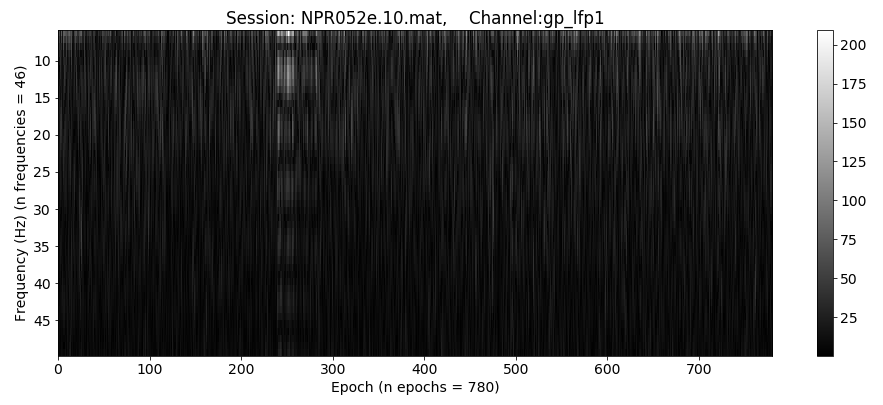
\includegraphics[width=1\textwidth]{images/GP1.png}}
    \caption{SFVs for Globus Pallidus LFP channel of a specific session.}
    \label{fig:GP1}
\end{figure}

\begin{figure}[H]
    \centering
    \centerline{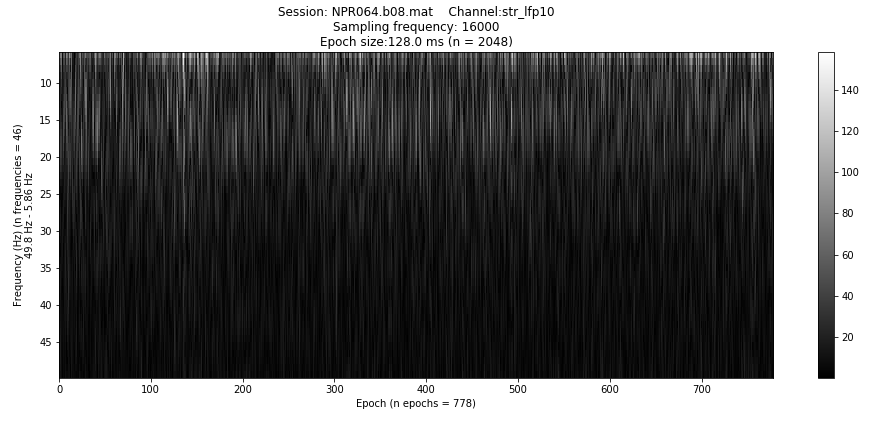
\includegraphics[width=1\textwidth]{images/STR2.png}}
    \caption{SFVs for Striatum LFP channel of a specific session.}
    \label{fig:STR2}
\end{figure}

\section{k-Means-based visualization}\label{KM Results}

Some of the produced k-Means prediction visualizations are shown in figures \ref{fig:KM4} and \ref{fig:KM16}.
In order to better relate to the heuristic argument presented in section \ref{KM Method}, the colors for class assignments were chosen to be sorted by the "sum of power spectrum" (sum of squares) of the cluster centers.
Lower class index (refer to color bar in either figure) represents lower sum of power spectrum.

In the figures, each row represents the class assignments for a specific channel in the set.
The columns represent epochs.
Each colored "slice" is the prediction of a single SFV to a class, the result of a trained k-Means model.
The particular channel names are not shown in these figures, but include both STR and GP channels, sorted such that channels 0 - 10 are GP channels and 11 - 14 are STR channels.
The SFVs are identical in production parameters to those presented in section \ref{SFV Results}.

The most important thing to note about these figures is how different channels in the same (or close) epochs tend to be given equal class assignments excessively. 
The authors interpret the class assignments for adjacent epochs to often be "close", meaning that class assignments seem to be followed by slightly higher or slightly lower class assignments (referring to class index), this was however not researched more thoroughly and should be considered an informal observation.
Also of note are "streaks" of higher class assignments for specific channels.
Channel 11, notably, has multiple such streaks.
Informally, there also appears to be a certain "verticality" to most epochs, where assignments over multiple channels are excessively similar at simultaneous times.

\begin{figure}[H]
    \centering
    \centerline{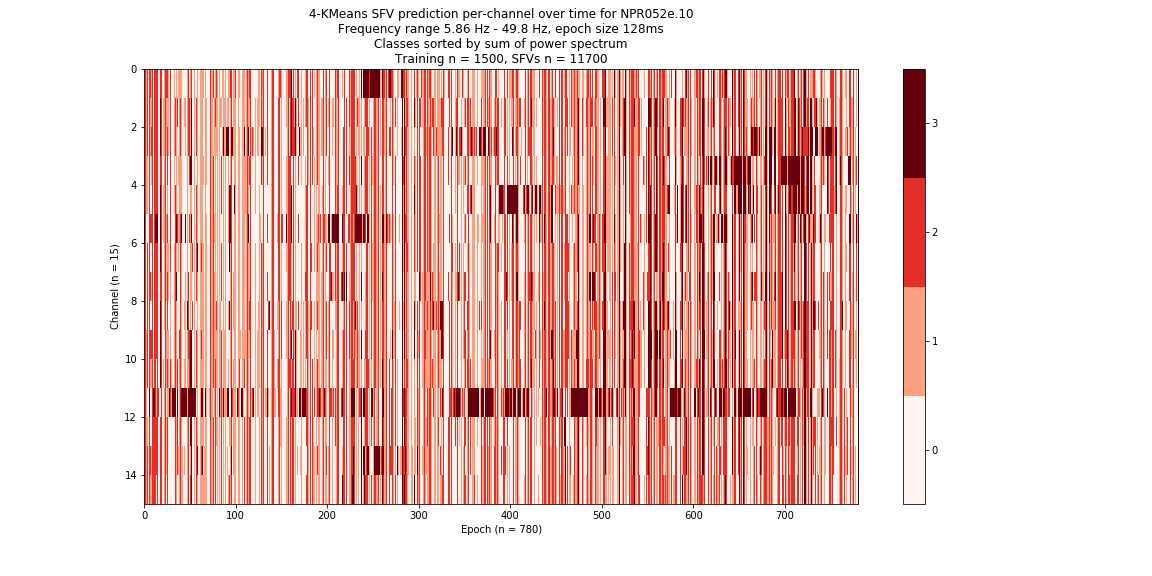
\includegraphics[width=1\textwidth]{images/KM4.png}}
    \caption{4-k-Means of channels for specific session.}
    \label{fig:KM4}
\end{figure}

\begin{figure}[H]
    \centering
    \centerline{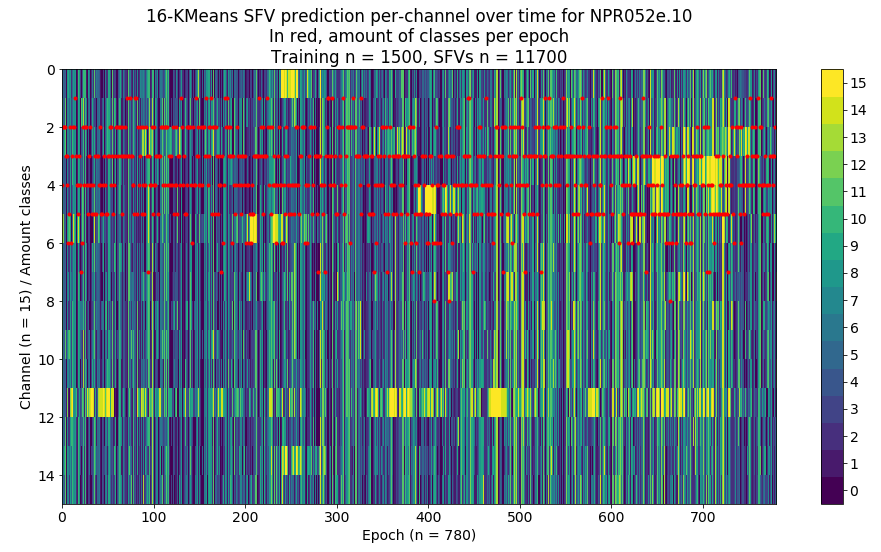
\includegraphics[width=1\textwidth]{images/KM16.png}}
    \caption{16-k-Means of channels for specific session.}
    \label{fig:KM16}
\end{figure}

\section{Principal component analysis of spectrum feature vectors}\label{PCA Results}

The method outlined in section \ref{PCA Methods} was performed using a set of 362,184 SFVs produced with parameters identical to those described in section \ref{SFV Results}.
Indeed, the SFVs shown in figures \ref{fig:GP1} and \ref{fig:STR2} are part of the set used to compute the PCA model.

The first thing to consider about the PCs computed for the set of SFVs are the PCs themselves.
Figure \ref{fig:PCS} shows these, as well as their respective explained variance ratios. 
In this specific case, eight PCs were produced, as this was the points where their cumulative sum of explained variance ratio was above 90\%.
A linear combination of these PCs can describe the entire set of SFVs with a great degree of accuracy.

\begin{figure}[H]
    \centering
    \centerline{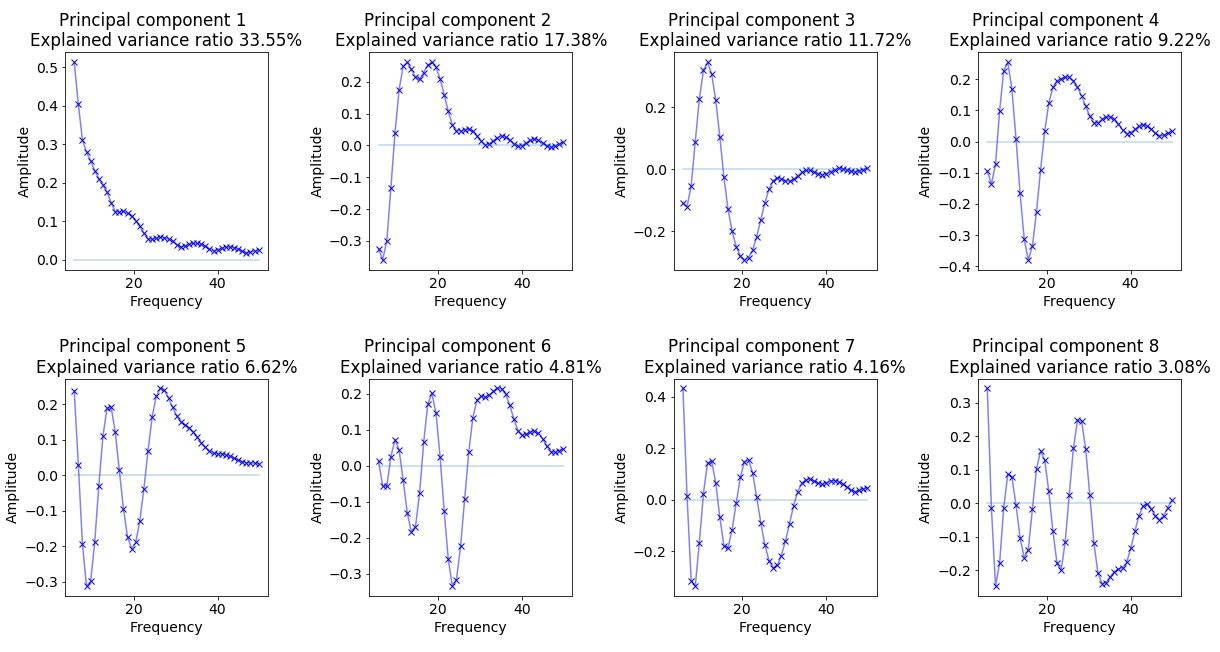
\includegraphics[width=1\textwidth]{images/PCA/PCS.png}}
    \caption{Principal components of SFV-set.}
    \label{fig:PCS}
\end{figure}

Having computed these PCs, the approximate probability distributions of the individual components as they appear in the set of "PCA-transformed" SFVs are shown in figure \ref{fig:PCAPDF}. 
In order to better visualize the long tails of these distributions, the probability distributions of the logarithms (base 2) of the individual components are shown in figure \ref{fig:PCAPDFLG2}.

\begin{figure}[H]
    \centering
    \centerline{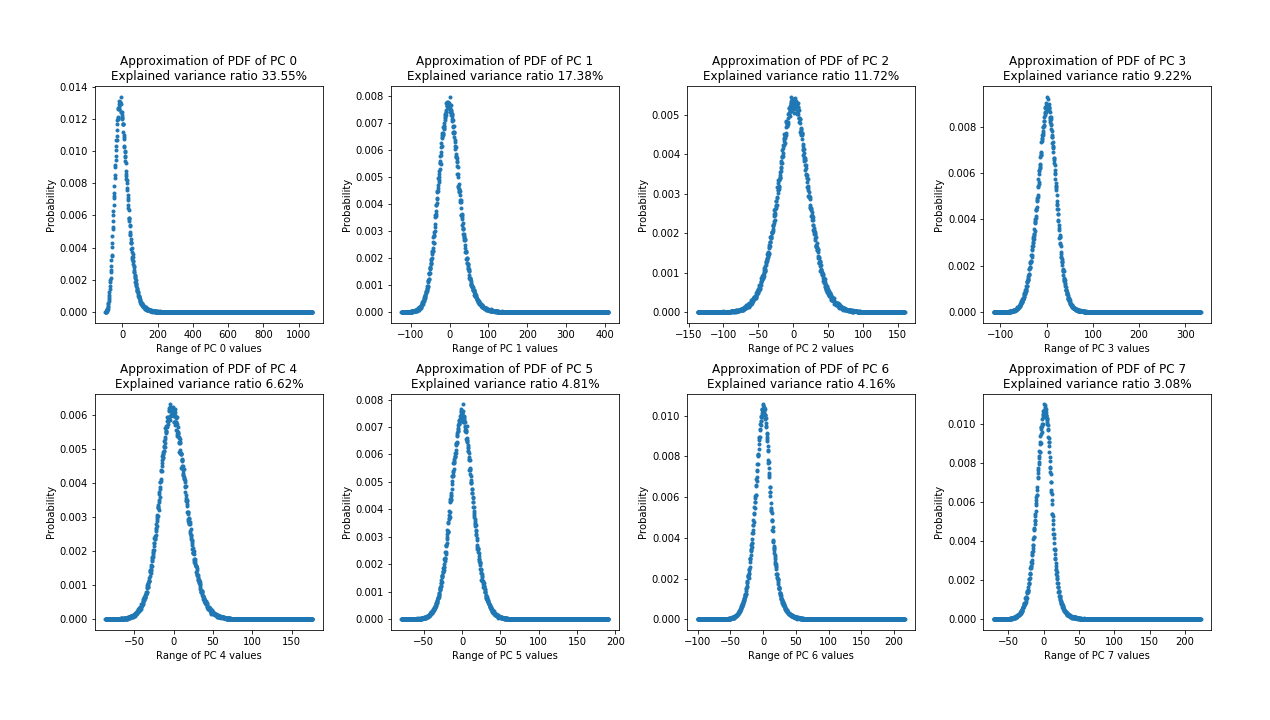
\includegraphics[width=1\textwidth]{images/PCA/PCAPDF.png}}
    \caption{Approximate distributions of principal components of SFV-set.}
    \label{fig:PCAPDF}
\end{figure}

\begin{figure}[H]
    \centering
    \centerline{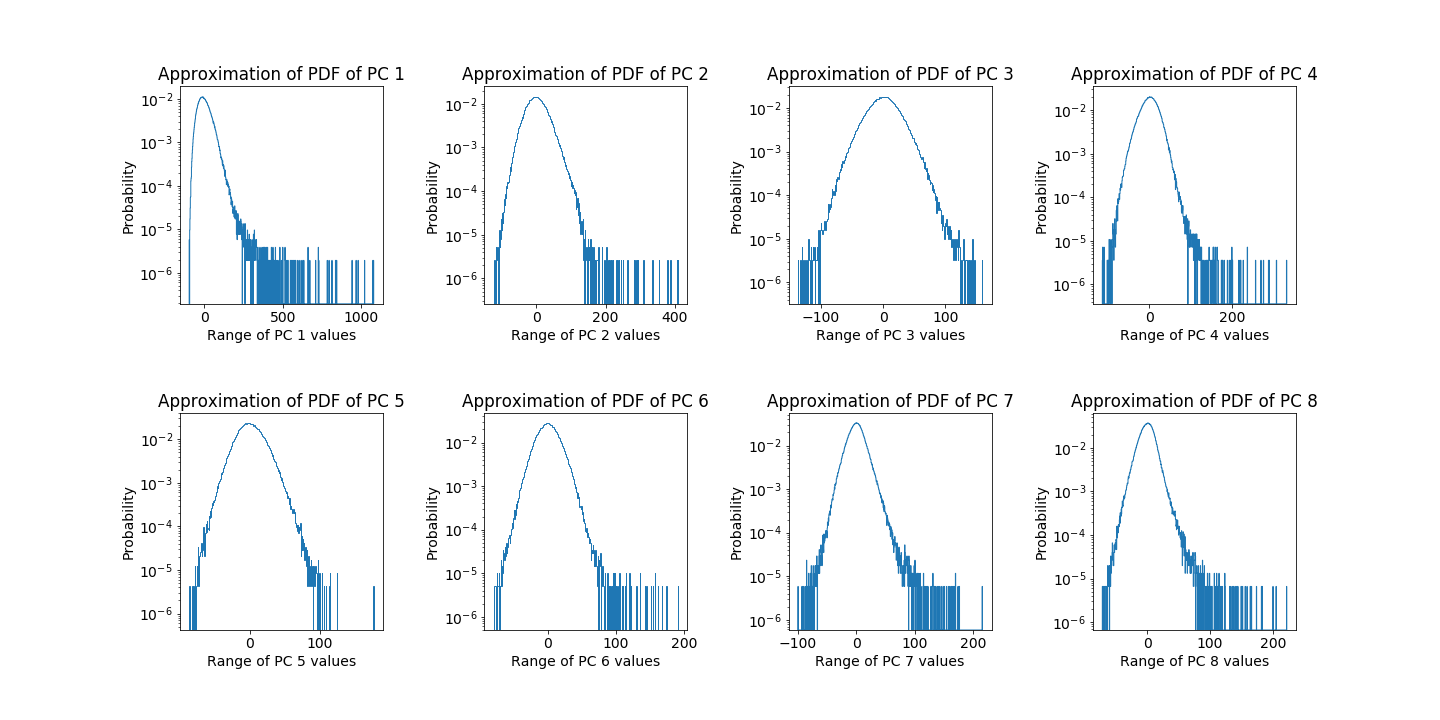
\includegraphics[width=1\textwidth]{images/PCA/PCAPDFLG2.png}}
    \caption{Approximate distributions of \begin{math}log_2\end{math} of principal components of SFV-set.}
    \label{fig:PCAPDFLG2}
\end{figure}

The information shown in figures \ref{fig:PCAPDF} and \ref{fig:PCAPDFLG2} is also shown in figures \ref{fig:PCAPDFBOTH} and \ref{fig:PCAPDFBOTHLG2}, except with channels from STR kept separate from those of GP.
Notably, GP channels exhibit distributions with more width and higher peaks.

\begin{figure}[H]
    \centering
    \centerline{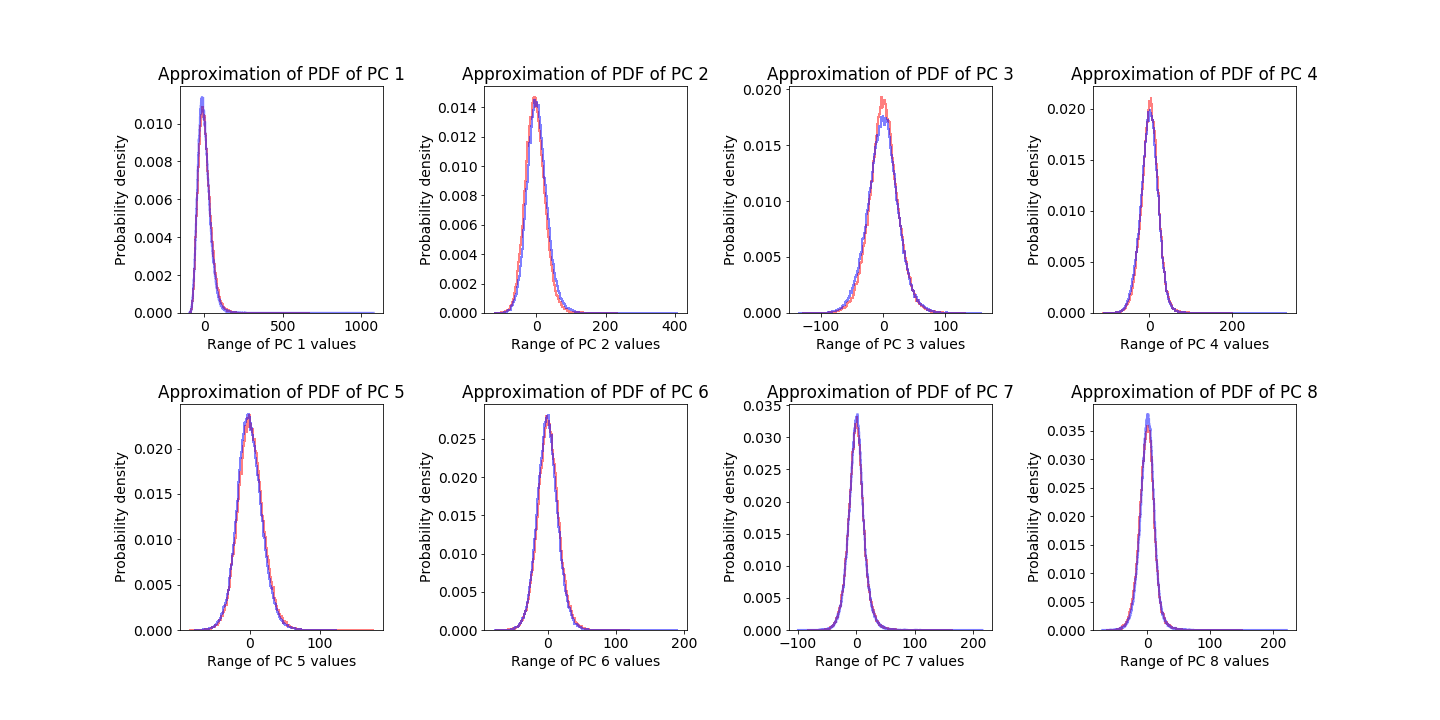
\includegraphics[width=1\textwidth]{images/PCA/PCABOTH.png}}
    \caption{Approximate distributions of principal components of SFV-set, separated by channel type.}
    \label{fig:PCAPDFBOTH}
\end{figure}

\begin{figure}[H]
    \centering
    \centerline{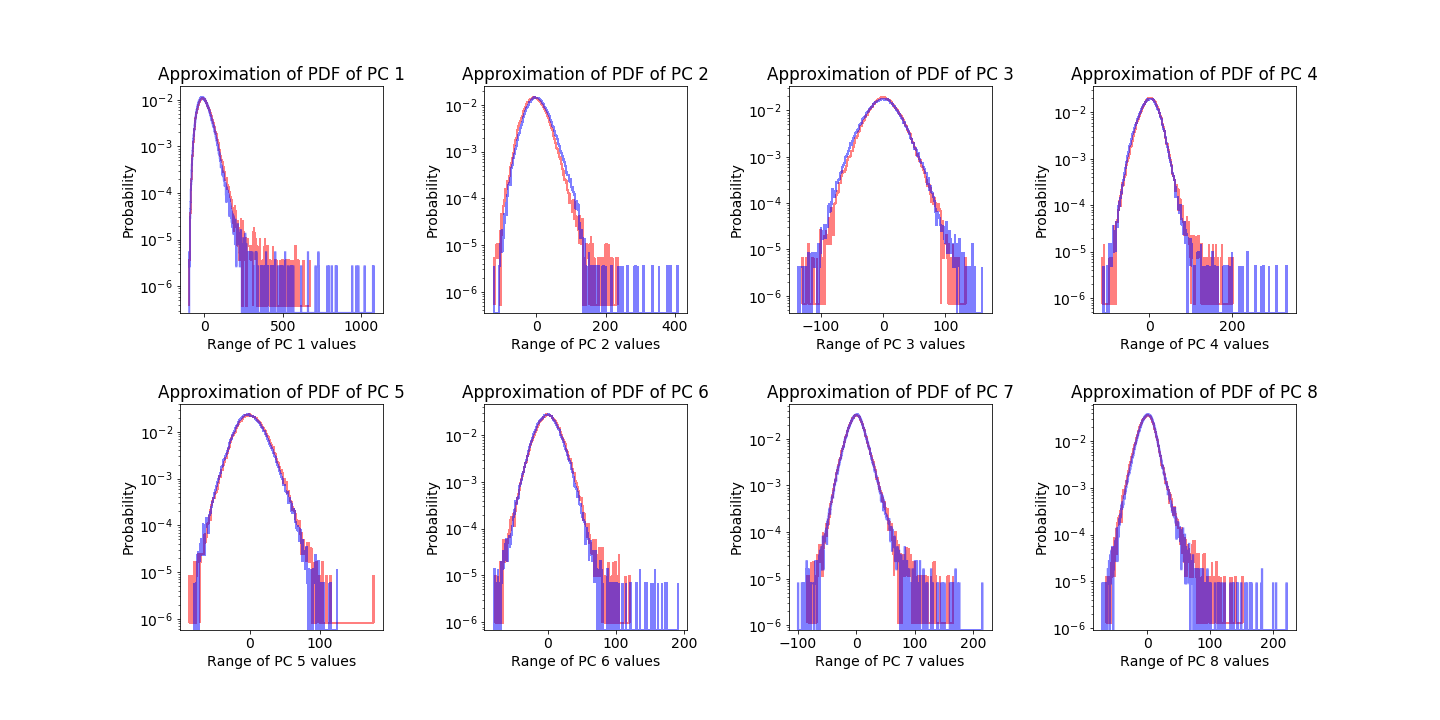
\includegraphics[width=1\textwidth]{images/PCA/PCABOTHLG2.png}}
    \caption{Approximate distributions of \begin{math}log_2\end{math} of principal components of SFV-set, separated by channel type.}
    \label{fig:PCAPDFBOTHLG2}
\end{figure}

Additionally, equivalent figures can be used to consider differences in the LFP activity of different animals, by producing the distributions (and differences of such) in different sessions.
Figures \ref{fig:PCAAnimals} and \ref{fig:PCAAnimalslg2} show such visualizations, for sessions \texttt{NPR-076.c09} in red, \texttt{NPR064.c09} in blue, and \texttt{NPR065e.03} in green.

\begin{figure}[H]
    \centering
    \centerline{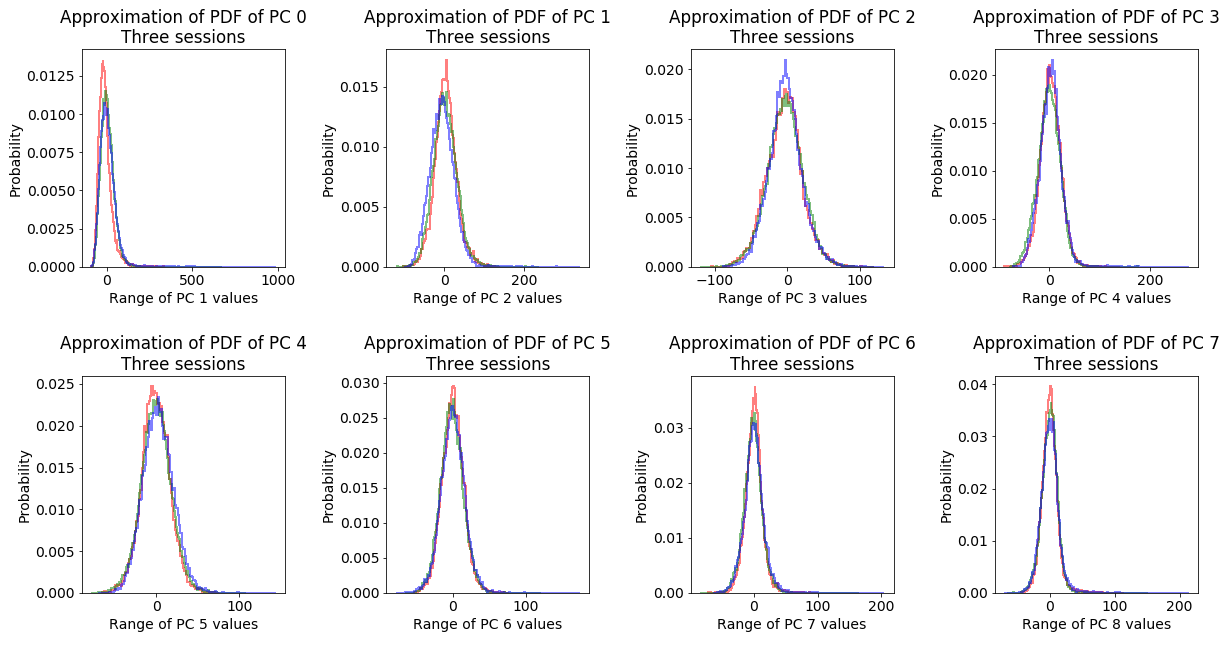
\includegraphics[width=1\textwidth]{images/PCA/PCAAnimalsnormal.png}}
    \caption{Approximate distributions of \begin{math}log_2\end{math} of principal components of SFV-set, separated by session.}
    \label{fig:PCAAnimals}
\end{figure}

\begin{figure}[H]
    \centering
    \centerline{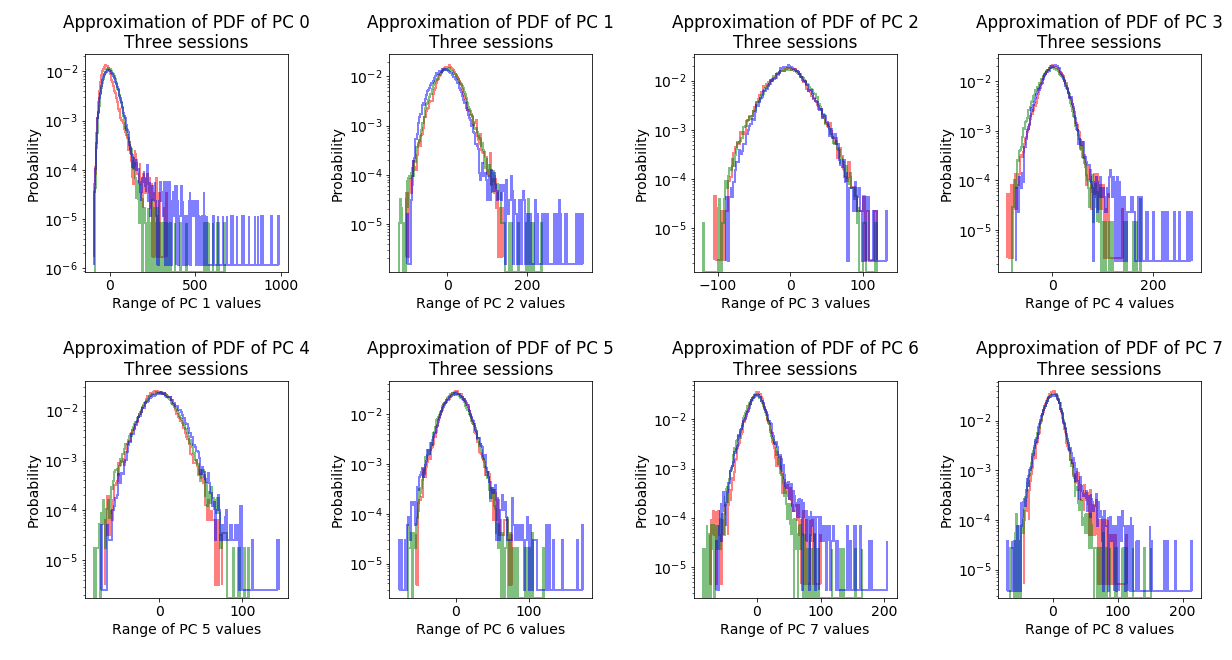
\includegraphics[width=1\textwidth]{images/PCA/PCAAnimalslg2.png}}
    \caption{Approximate distributions of \begin{math}log_2\end{math} of principal components of SFV-set, separated by session.}
    \label{fig:PCAAnimalslg2}
\end{figure}

These figures, of course, don't show how these distributions correlate.
Tables \ref{tab:corrcoefGP} and \ref{tab:corrcoefSTR} show the cross-correlations of PCs of "PCA-transformed" SFVs, for GP and STR channels respectively.
Notably, cross-correlation within STR channels is consistently low, while it is consistently considerably higher within GP channels.

\begin{table}[H]
    \centering
    \begin{tabular}{|c|c|c|c|c|c|c|c|c|}
    \hline
          & PC 0 & PC 1 & PC 2 & PC 3  & PC 4 & PC 5 & PC 6 & PC 7 \\ \hline
     PC 0 & 1.0  & 0.43 & 0.17 & 0.44  & 0.23 & 0.39 & 0.44 & 0.5  \\ \hline
     PC 1 & 0.43 & 1.0  & 0.1  & 0.26  & 0.13 & 0.26 & 0.26 & 0.31 \\ \hline
     PC 2 & 0.17 & 0.1  & 1.0  & 0.11  & 0.07 & 0.08 & 0.12 & 0.13 \\ \hline
     PC 3 & 0.44 & 0.26 & 0.11 & 1.0   & 0.16 & 0.26 & 0.31 & 0.35 \\ \hline
     PC 4 & 0.23 & 0.13 & 0.07 & 0.16  & 1.0  & 0.13 & 0.16 & 0.19 \\ \hline
     PC 5 & 0.39 & 0.26 & 0.08 & 0.26  & 0.13 & 1.0  & 0.27 & 0.32 \\ \hline
     PC 6 & 0.44 & 0.26 & 0.12 & 0.31  & 0.16 & 0.27 & 1.0  & 0.35 \\ \hline
     PC 7 & 0.5  & 0.31 & 0.13 & 0.35  & 0.19 & 0.32 & 0.35 & 1.0  \\ \hline
    \end{tabular}
    \caption{Cross-correlation of PCs, GP channels, rounded to two decimals.}
    \label{tab:corrcoefGP}
\end{table}

\begin{table}[H]
    \centering
    \begin{tabular}{|c|c|c|c|c|c|c|c|c|}
    \hline
          & PC 0  &  PC 1 &  PC 2 &  PC 3 &  PC 4 &  PC 5 &  PC 6 &  PC 7 \\ \hline
     PC 0 &  1.0  & -0.05 &  0.01 &  0.0  &  0.0  & -0.01 & -0.0  &  0.01 \\ \hline
     PC 1 & -0.05 &  1.0  &  0.05 &  0.08 &  0.03 &  0.01 &  0.04 &  0.03 \\ \hline
     PC 2 &  0.01 &  0.05 &  1.0  &  0.03 & -0.02 &  0.02 &  0.02 & -0.01 \\ \hline
     PC 3 &  0.0  &  0.08 &  0.03 &  1.0  & -0.0  &  0.03 & -0.02 &  0.01 \\ \hline
     PC 4 &  0.0  &  0.03 & -0.02 & -0.0  &  1.0  &  0.01 &  0.01 & -0.0  \\ \hline
     PC 5 & -0.01 &  0.01 &  0.02 &  0.03 &  0.01 &  1.0 &  -0.0  & -0.01 \\ \hline
     PC 6 & -0.0  &  0.04 &  0.02 & -0.02 &  0.01 & -0.0 &   1.0  &  0.0  \\ \hline
     PC 7 &  0.01 &  0.03 & -0.01 &  0.01 & -0.0  & -0.01 &  0.0  &  1.0  \\ \hline
    \end{tabular}
    \caption{Cross-correlation of PCs, STR channels, rounded to two decimals.}
    \label{tab:corrcoefSTR}
\end{table}

\section{Spiking analysis results}

This section is dedicated to the results of analysis of spiking rate data, by methods described in 
All results are produced taking 50 successive time windows of 0.5 seconds each.

\subsection{Spiking rates}

Figure \ref{fig:ratesBoth1} shows the spiking rate functions of the channels of both regions (channels 0-6 are from the GP, channels 7-16 are from the STN). Rows represent channels and columns represent time windows. 

\begin{figure}[H]
    \centering
    \centerline{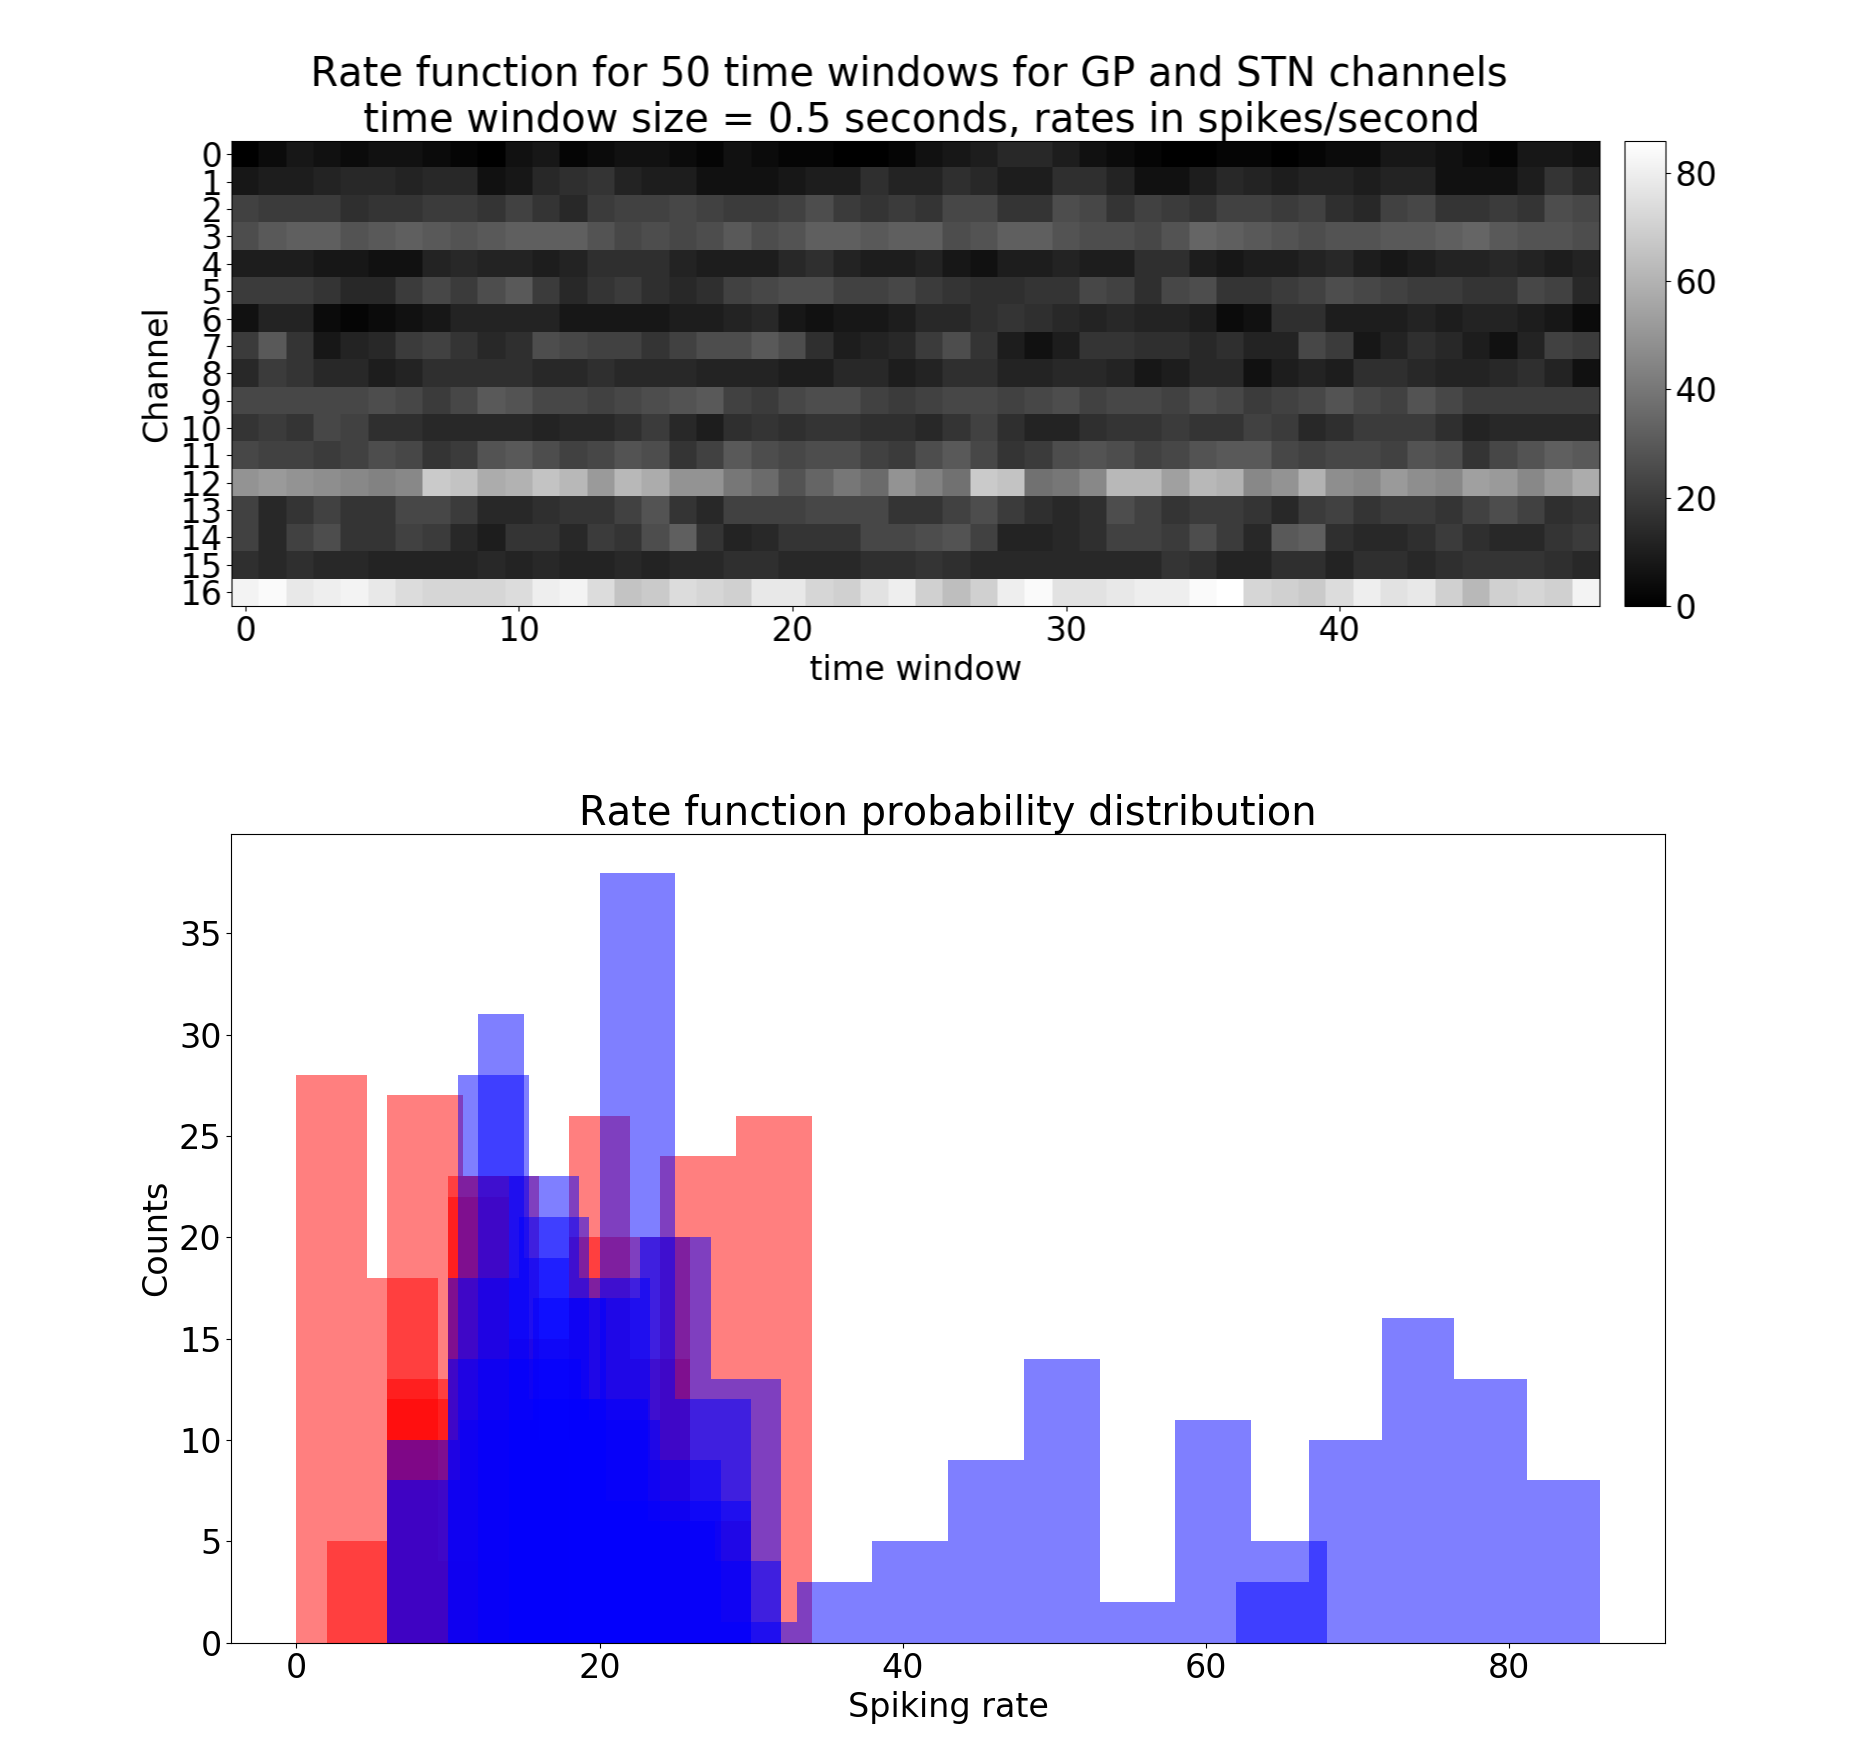
\includegraphics[width=1\textwidth]{images/spiking/SR_all.png}}
    \caption{Spiking rates of GP and STN channels.}
    \label{fig:ratesBoth1}
\end{figure}

\subsection{Joint rate distributions}

The data is displayed in the form of scatter diagrams, in which the sequence of firing rates (represented by the abscissa) is plotted against the same sequence with a lag of one time window (represented by the ordinate). 
Each point on the diagram then represents a pair of “adjacent” rates.

The hexagonal scatterplots are better at showing the density of the overall joint distribution, whereas the normal ones differentiate among channels (in the case they are all from the same region), or among regions (if both regions are plotted together).

Figure \ref{fig:JP1} and figure \ref{fig:JP2} respectively show the joint probability distributions of the channels in the GP and STN, whereas figure \ref{fig:JP3} displays the joint distribution of every channel in both regions. 
In the non-hexagonal scatterplots, there is one color per channel (in the case of Figure 1 and 2), or red for GP and blue for STN (in Figure 3).

\begin{figure}[H]
    \centering
    \centerline{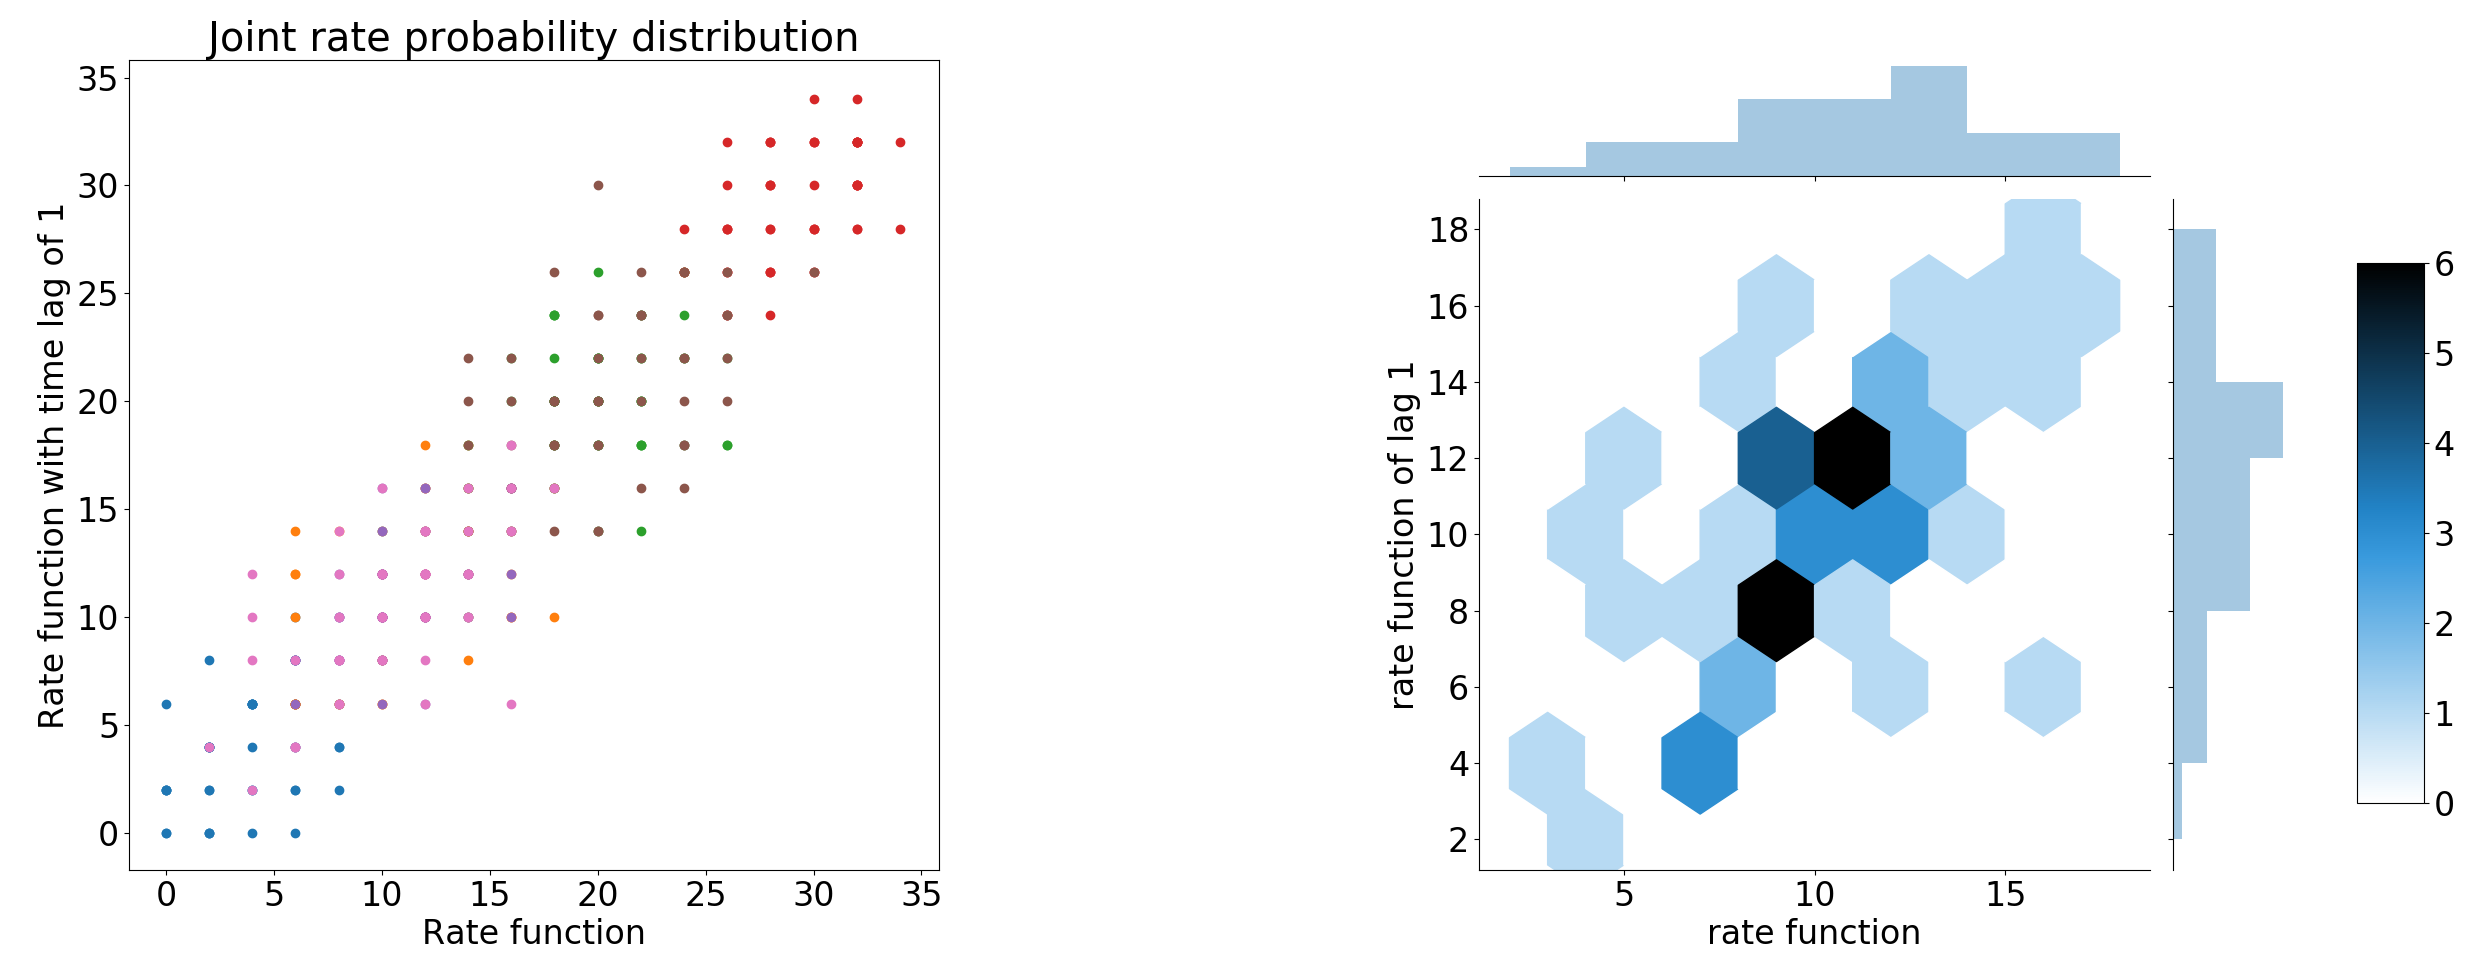
\includegraphics[width=1\textwidth]{images/spiking/JP_gp.png}}
    \caption{Joint probability distribution of the spiking rates of all GP channels and these same sequences with a time lag of one window. }
    \label{fig:JP1}
\end{figure}

\begin{figure}[H]
    \centering
    \centerline{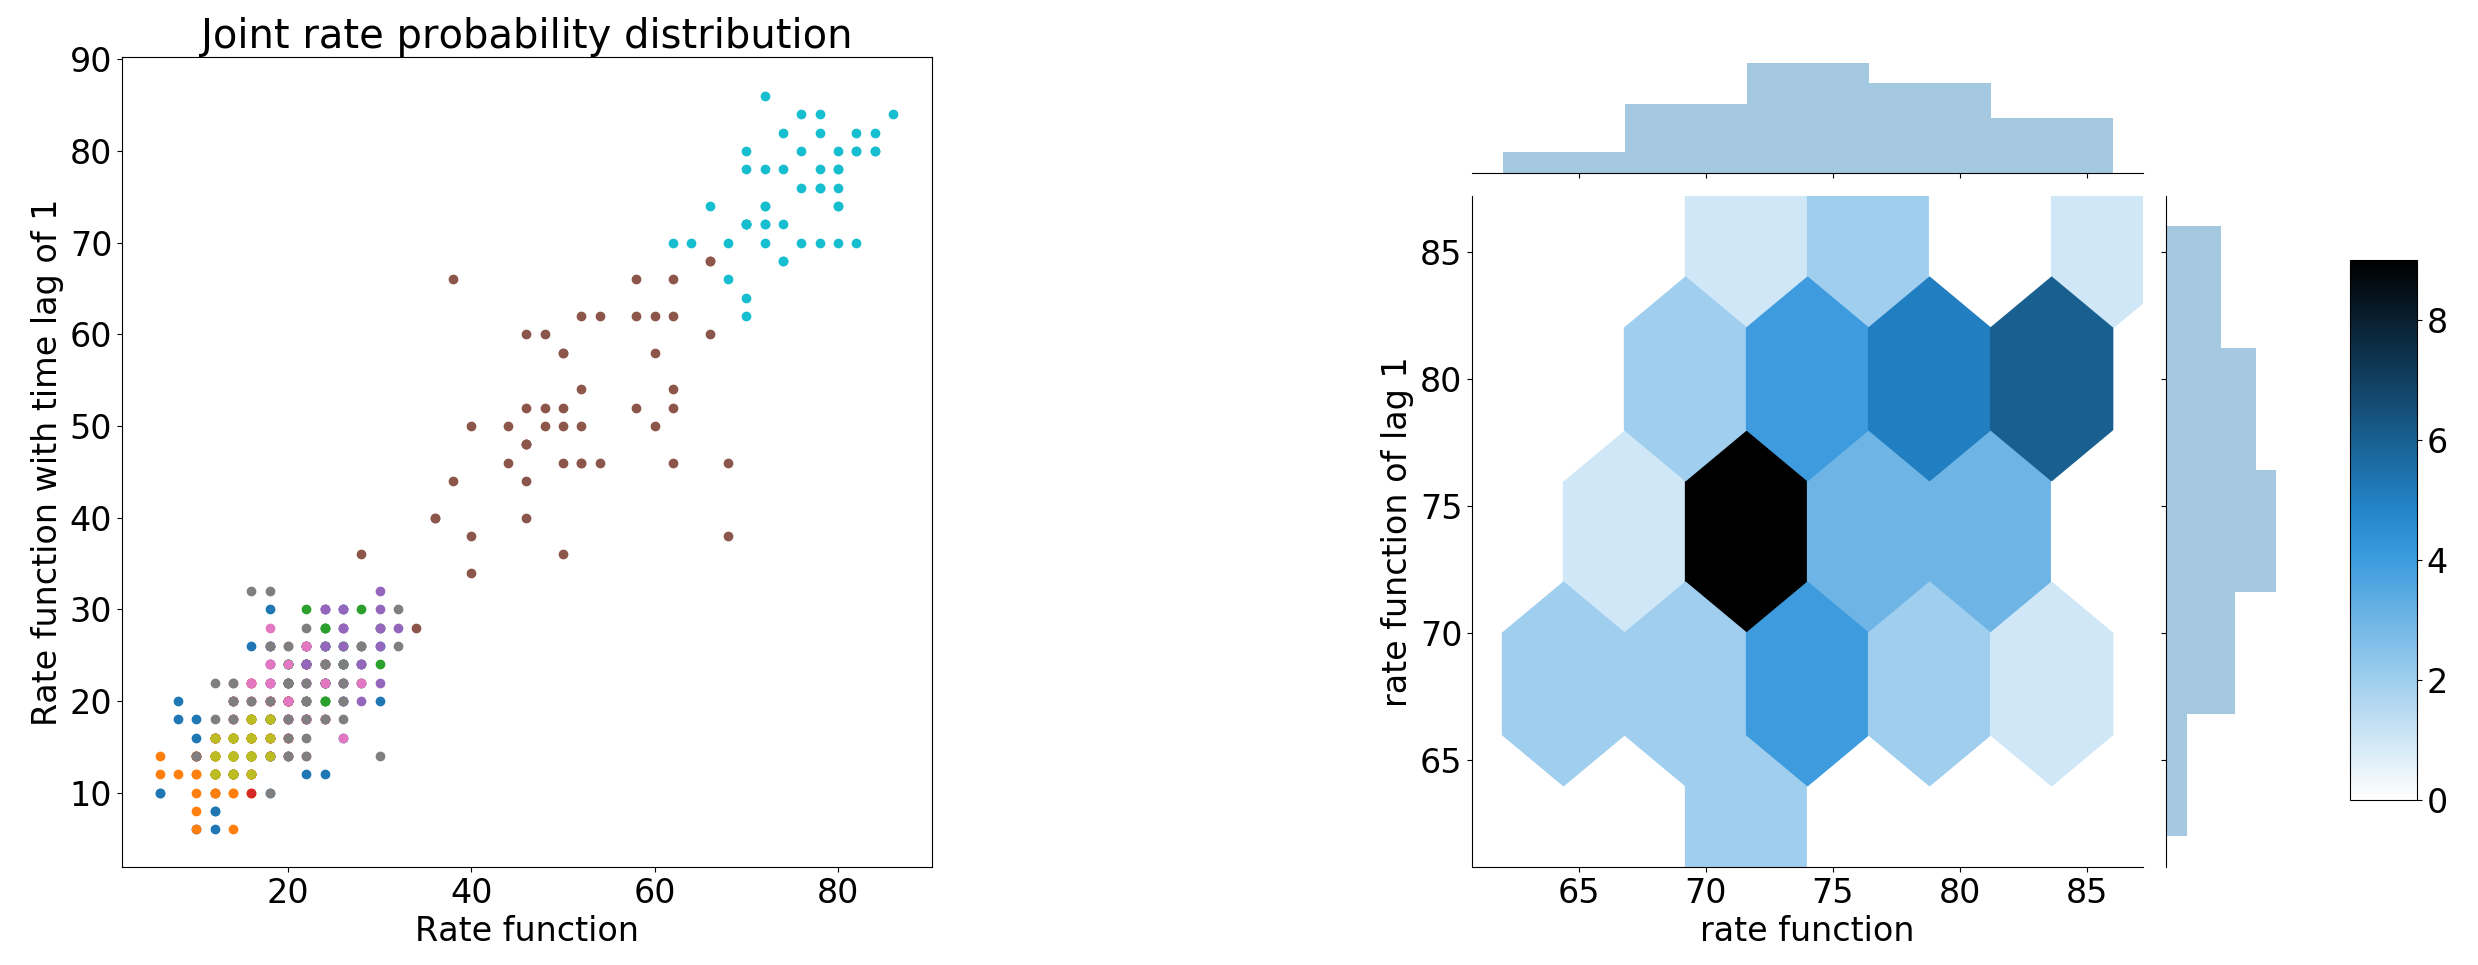
\includegraphics[width=1\textwidth]{images/spiking/JP_stn.png}}
    \caption{Joint probability distribution of the spiking rates of all STN channels and these same sequences with a time lag of one window.}
    \label{fig:JP2}
\end{figure}

\begin{figure}[H]
    \centering
    \centerline{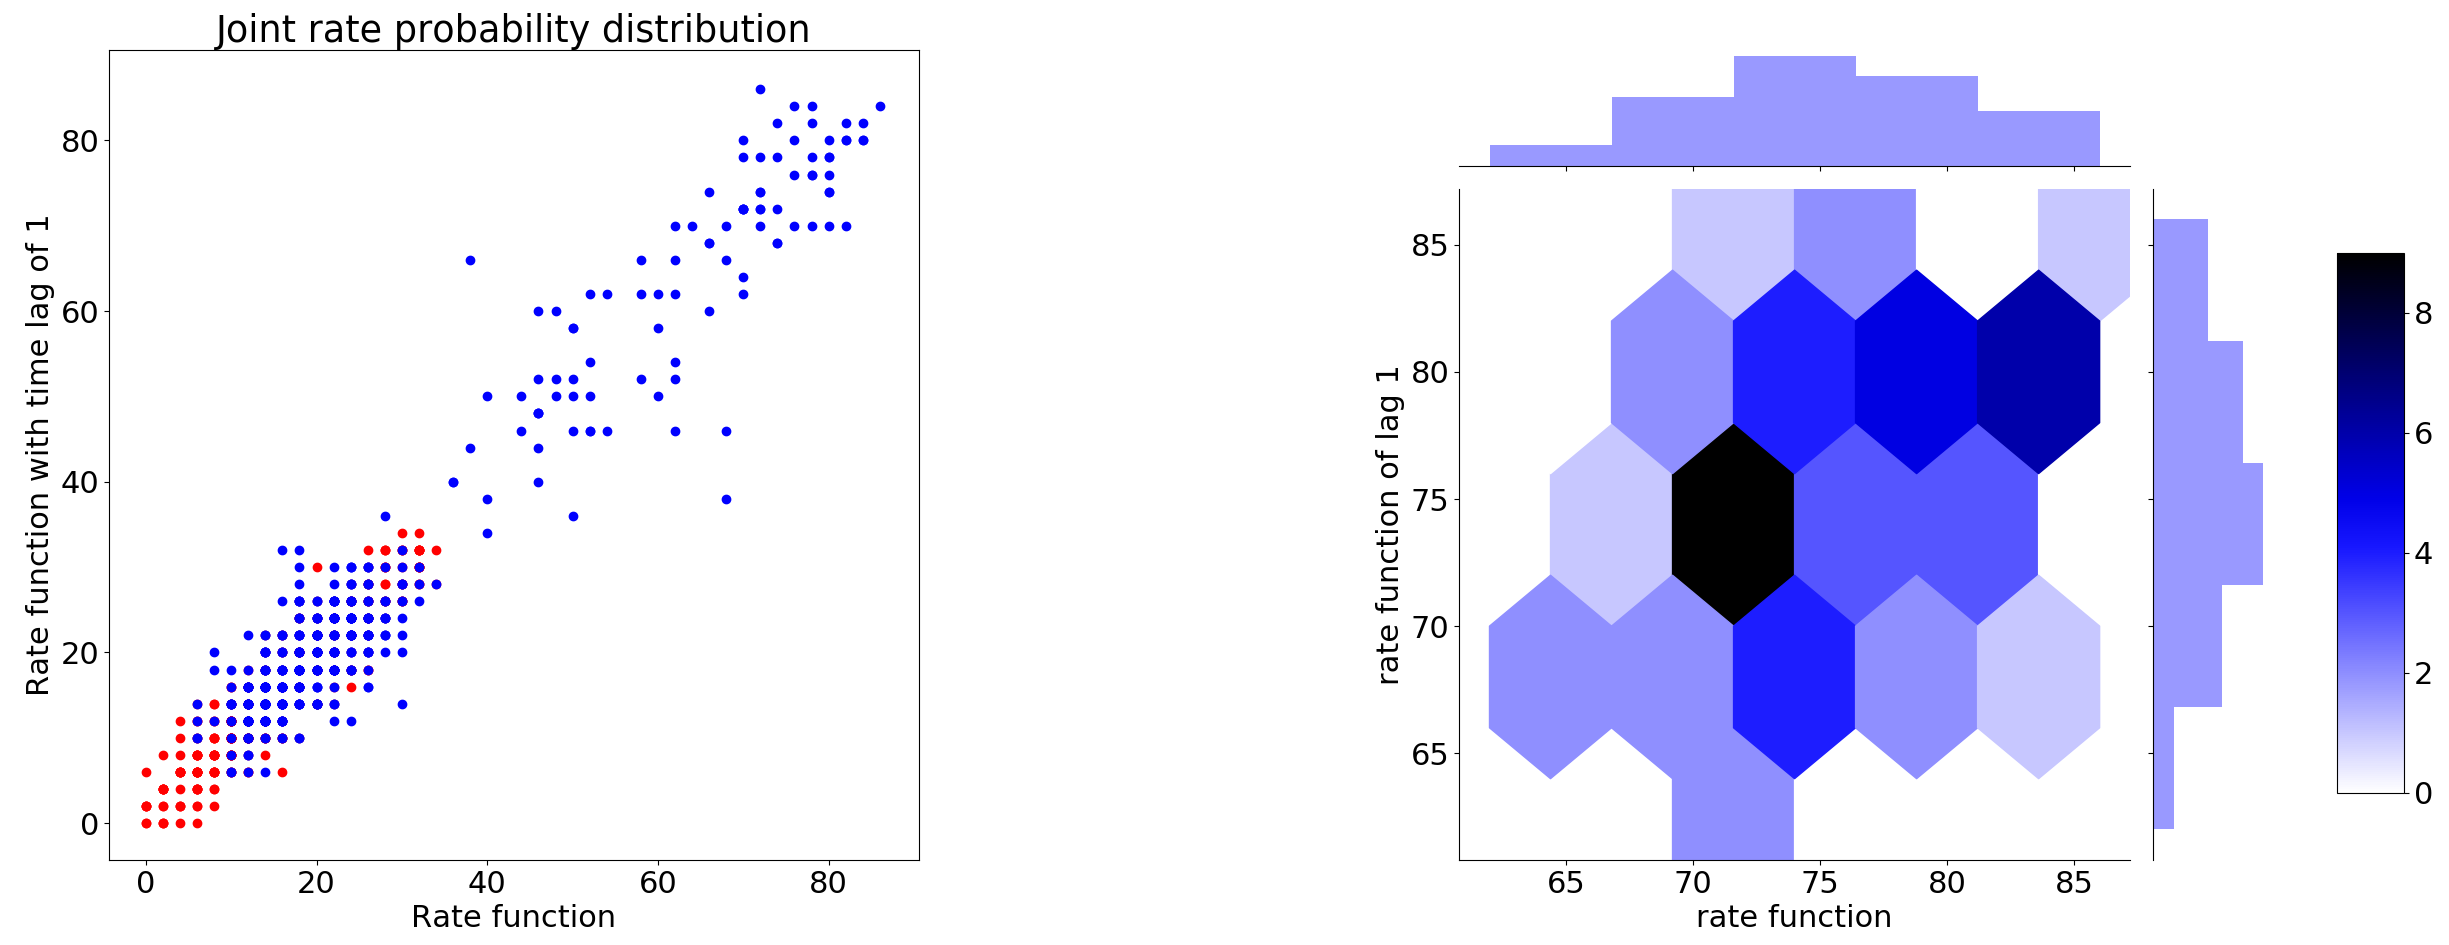
\includegraphics[width=1\textwidth]{images/spiking/JP_all.png}}
    \caption{Joint probability distribution of the spiking rates of all channels in the GP and STN regions and these same sequences with a time lag of one window.}
    \label{fig:JP3}
\end{figure}

\subsection{Serial correlation coefficients}

Figure \ref{fig:corr3} shows the same information for all channels. Channels 0-6 are from GP, channels 7-16 are from STN
Rows represent channels and columns represent time windows.

\begin{figure}[H]
    \centering
    \centerline{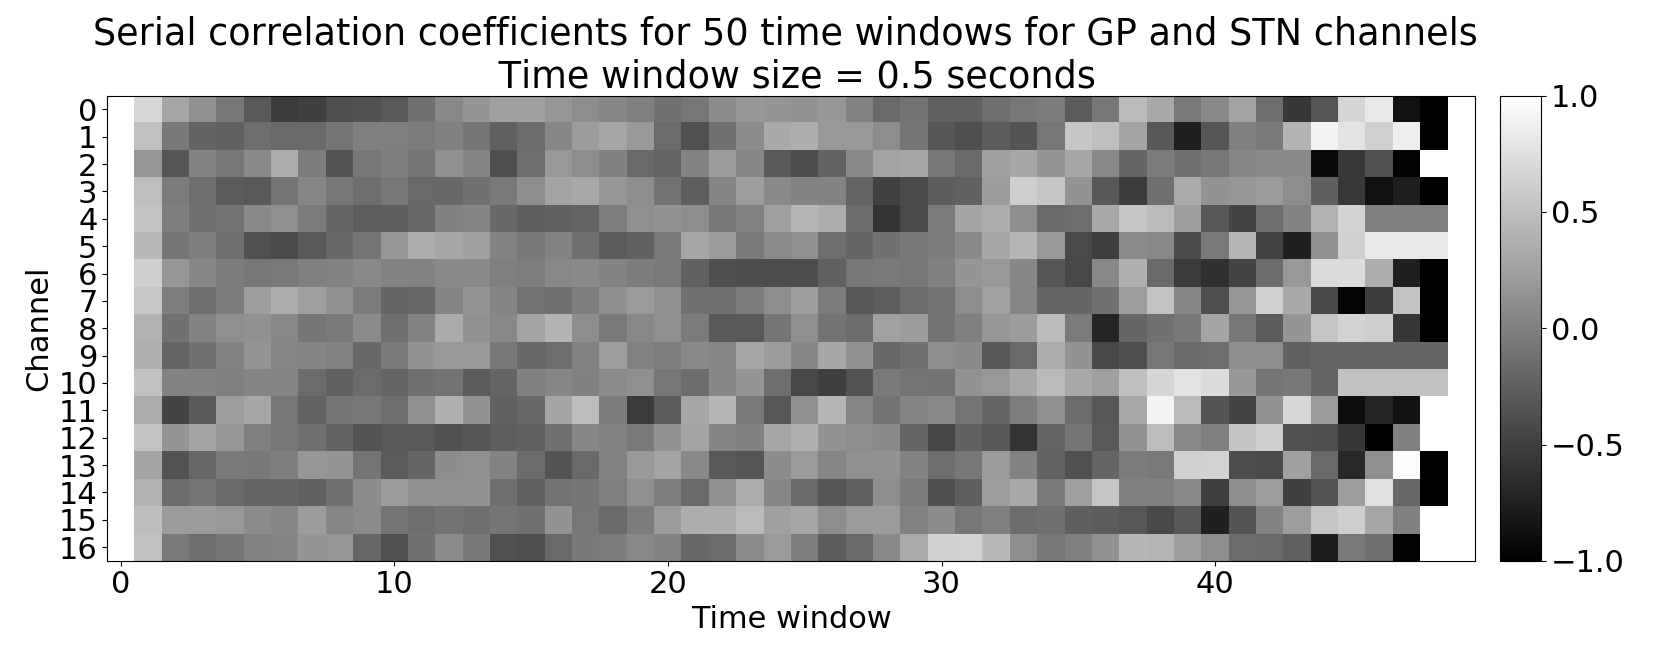
\includegraphics[width=1\textwidth]{images/spiking/autocorr_all.png}}
    \caption{Serial correlograms of all channels in the GP and STN.}
    \label{fig:corr3}
\end{figure}

\subsection{Power spectral density}

Figure \ref{fig:PS3} shows the power spectrum of both regions (red for GP, blue for STN).
The original spike data was recorded with a sampling frequency of 1 Hz, so the maximum frequency that is observable is 1 Hz.

\begin{figure}[H]
    \centering
    \centerline{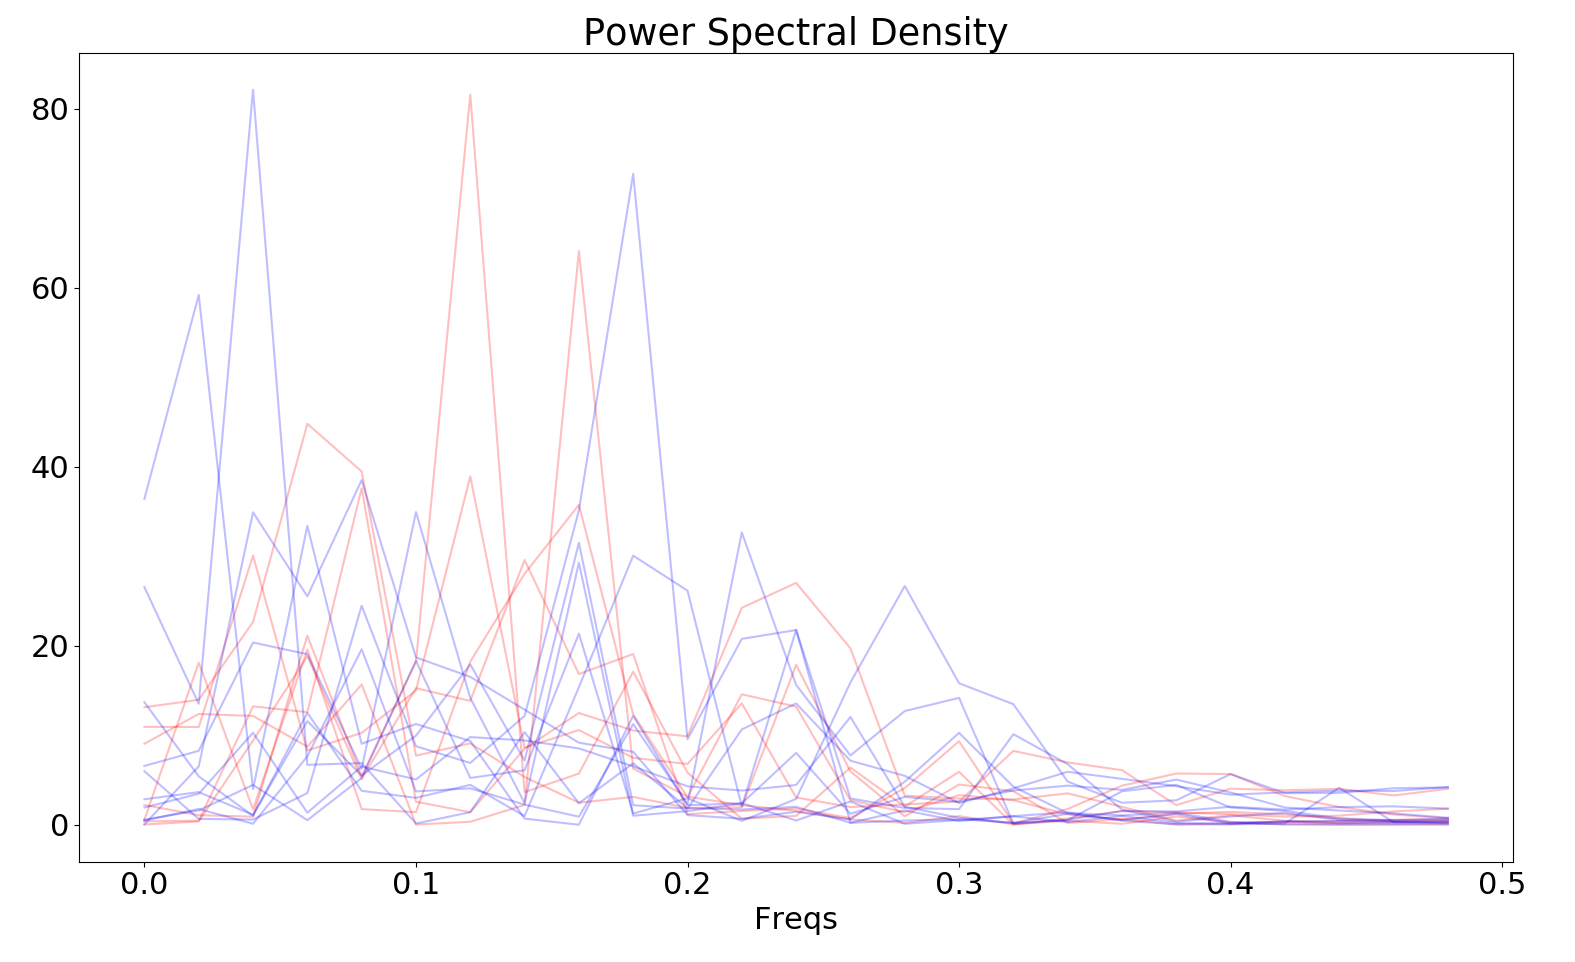
\includegraphics[width=1\textwidth]{images/spiking/powerSpect_all.png}}
    \caption{Power spectral density of all channels in the GP and STN.}
    \label{fig:PS3}
\end{figure}

\subsection{Spectral entropies}

Table \ref{tab:spec_entr} shows spectral entropies of select channels (channels 0-6 from the GP, channels 7-16 from the STN).

\begin{table}[H]
    \centering
    \begin{tabular}{|c|c|}
    \hline
                & Spectral Entropy \\ \hline
     Channel 0  & 0.793132         \\ \hline
     Channel 1  & 0.898098         \\ \hline
     Channel 2  & 0.827477         \\ \hline
     Channel 3  & 0.662636         \\ \hline
     Channel 4  & 0.619199         \\ \hline
     Channel 5  & 0.740590         \\ \hline
     Channel 6  & 0.778742         \\ \hline
     Channel 7  & 0.903068         \\ \hline
     Channel 8  & 0.804082         \\ \hline
     Channel 9  & 0.852935         \\ \hline
     Channel 10 & 0.638416         \\ \hline
     Channel 11 & 0.719677         \\ \hline
     Channel 12 & 0.752660         \\ \hline
     Channel 13 & 0.863742         \\ \hline
     Channel 14 & 0.798566         \\ \hline
     Channel 15 & 0.594042         \\ \hline
     Channel 16 & 0.832410         \\ \hline
    \end{tabular}
    \caption{Spectral entropies of select channels.}
    \label{tab:spec_entr}
\end{table}

\newpage
\chapter{Discussion}

This chapter is dedicated to discussion and interpretation of the produced results in the context of the research questions for this project.

\section{LFP activity based methods of classification}

This section discusses the methods described in sections \ref{DFT Method}, \ref{KM Method}, and \ref{PCA Methods}, with respective results in sections \ref{SFV Results}, \ref{KM Results}, and \ref{PCA Results}.

The authors believe that SFVs, as described in this report, are an appropriate means of feature extraction in the context of this report. 
This is not intended to be a proclamation of a groundbreaking discovery.
Analyzing the spectrum of brain activity has previously shown interesting results \parencite{Cagnan}, and SFVs are just a generalized approach to describe the process of extracting such spectra, taking fidelity, epoch size, and range of spectra into account.
Indeed, SFVs or similar methods have likely been described or used previously with a different name in previous research, not necessarily in this field of research.
SFVs also provide a simple mean of visualizing LFP activity in a human-understandable way.

To a layman in the study of neuroscience, the k-Means visualization heuristic applied in this project seems reasonable.
The results produced show LFP activity being strikingly similar for different areas of the basal ganglia when compared simultaneously.
Furthermore, the "outliers" present in figures \ref{fig:KM4} and \ref{fig:KM16} make intuitive sense, as one would expect outliers in any dataset.
This intuition, to reiterate, is that of a layman.
The authors imagine their chosen method and produced results may have serious flaws.
The authors, however, consider these results to at least be a reason to consider more sophisticated methods to attempt to cluster SFVs.
Such methods fall outside both the scope of this project, and the expertise of its' authors.

The authors believe that the produced PCs, or more specifically the method by which they were produced, show great potential for similar methods in the use of classification.
As discussed, the authors consider SFVs a reasonable means of feature extraction, and PCA proved effective in further investigating these.
A much smaller set of PCs than the number of features of their parent SFVs can describe them with great accuracy.
These PCs could then reasonably be interpreted, in the quite literal sense, as components making up LFP activity.
The PCs themselves could lend themselves to study and interpretation by more experienced scholars.
The rather extreme discrepancies between the nature of the distributions of these PCs when comparing GP channels to STR channels (see figures \ref{fig:PCAPDF}, \ref{fig:PCAPDFLG2}, tables \ref{tab:corrcoefGP}, \ref{tab:corrcoefSTR}) could also lend insight into the workings of these different brain regions.
Notable are the consistently lesser amplitudes of activity in STR, and the consistently much lower cross-correlation of PCs in STR.
While the PCs described in figure \ref{fig:PCS} are present almost independently in STR channels, they have clear correlation in GP channels.
Interpreting this is beyond the experience of the authors.

\section{Spiking rate based methods of classification}

The model used to analyse spikes provides a set of measurements in both time and spectral domains that are used to attempt an observation of the distinctions in a broad collection of spiking activity data. These properties cannot be understood isolated, but related to each other. The measurements were taken in order to examine the spiking activity of the STN and GP regions, since the STN-GP network is relevant for PD, and to know whether there are differences in the activity of both regions. The results remain of interest even if their activity is finally found to be similar. Relying on previous research, another aim is to note a big degree of complexity or disorder in all channels, which belongs to a Parkinsonian state.

\subsection{Spiking rates}

With regard to the spiking rates that were obtained, no clear distinctions can be drawn between different regions, since their spiking rates remain within a range that stays constant across channels, except for two individual channels in the subthalamic nucleus that show significantly higher values. On the plots, a not entirely explicit but moderately identifiable firing pattern for each channel can be seen, with semi-regular spiking bursts (periods of time where the neuron fires more frequently). 

The scatter diagrams of adjacent rates do show differences among channels and especially regions, which can be very clearly distinguished from each other. The spiking rate of the neurons in the STN varies in a range which is higher than those in the GP. 
These scatter diagrams may provide the best insight on how successive spiking rates relate and depend on each other. Although the serial correlation coefficients allow a quantification of the time-dependent correlation of rates, they are not so useful to identify any inherent patterns in the scattergrams; identifying and quantifying in terms of density the clustered structures in such scattergrams is instead a better solution. 
Departures from independence between spiking rates are reflected in the symmetries of the scatter diagram itself. The diagrams show an overall upward trend, which indicates positive correlations between successive rates. That loosely means that short intervals between consecutive spikes tend to be followed by short ones, and long intervals by long ones. A downward trend would mean the opposite.
Not taking into account all the available time windows when making the calculations is more convenient to see more specific dissimilarities among channels. Drawing results from a smaller time frame, for example 50 windows, allows to identify channels that are more “silent” than others at a certain range of time, as can be seen in the scattergrams that differentiate each channel with a colour. 

\subsection{Spectral properties of the spike count sequences}

Apart from properties in the time domain, other complex properties are present in basal ganglia spike sequences, like those in the spectral domain. Based on the power spectrums of the autocorrelation of the channels, an evident synchronization between the globus pallidus and subthalamic nucleus can be observed; both regions share similar power spectrograms, and the peaks in frequency stay within the same range of values; the estimated frequencies with the highest amount of variance (or noise) are between the values [0, 0.05] and [0.1, 0.2], and are common across all channels. Referring to the implications of noise on signal transmission theory which were mentioned in early sections, a high noise at a certain frequency is a limiting factor to information transmission between neurons at that frequency. 

The spectral entropy values are then useful to quantify the general level of disorder or noise of each channel, based on the power spectrums. When computing the spectral entropies in bins of 25 time windows, both regions vary in the same way over time, and their estimated probability distributions are similar. Likewise, when calculating the spectral entropies using all 393 time windows, the values show no significant differences between the spectral entropies in the GP and those in the STN. They are all evenly distributed, and it can be affirmed that all channels have generally high spectral entropies going from approximately 0.6 to 0.9 (with 1 being the highest possible value). Despite having a high quantity of noise, they still have a small level of predictability. 


\newpage
\chapter{Conclusion}

\textbf{This section is not at the same level of completion as previous sections.}

The methods produced for classifying Parkinson's disease based on LFP activity show potential.
While results shown have often been comparing e.g. categories of channels, or the activity within a single session, much of this can be generalized.
Larger datasets could be used, and subjects could be compared instead of channel categories (and vice versa).
More extensive and sophisticated attempts at interpreting the use and results of the methods developed could be undertaken, and additional regions of the brain could be considered.
It's likely that many additional avenues for further research could be explored, that are outside the imaginations of the authors.

The authors believe that the methods and results developed based on LFP activity in the basal ganglia for the purpose of classification of Parkinson's disease show definitive potential for future research.

\newpage
\printbibliography[heading=bibintoc]

\end{document}